%%%% This Beamer example was created by LianTze Lim, April 2017.

%%%% This is a VERY simple and minimalistic beamer theme,
%%%% even reminiscent of marker pens on transparencies!
%%%% It mimics the look of the "seminar" package, which
%%%% can only be used with plain TeX.
%%%% There are also some comments and example to show how
%%%% to customise various elements, e.g. the font and colours.

\documentclass[12pt]{beamer}
%% If you'd like the default font size to be even larger, use 14pt or 17pt; these are supported by Beamer.

\usepackage[english]{babel}
\usepackage[utf8]{inputenc}
\usepackage[T1]{fontenc}
\usepackage{lmodern}
\usepackage{tikz}


%%%%%%%%%%%%%%%%%%%%%%%%%%%%%%%%%%%%%%%%%
% These lines should usually go into a .sty file,
% but I'll leave them here so that it's easier to
% see how to customise a Beamer theme.
% Remember, the Beamer manual is your friend!!
% http://texdoc.net/pkg/beamer
%
%% So if your re-definitions have a @ somewhere, you
%% _MUST_ put a \makeatletter before these lines and then
%% \makeatother after them. This trick can only be done
%% in the preamble! BUT if you're doing these re-definitions
%% in a .sty file (so that you \usepackage it later), you
%% don't need the \makeatletter and \makeatother.
\makeatletter

%% Set the left and right margins
\setbeamersize{text margin left=1em,text margin right=1em}

%% FONTS
\setbeamerfont{title}{series=\bfseries,size=\LARGE}
\setbeamerfont{subtitle}{series=\bfseries,size=\Large}
\setbeamerfont{frametitle}{series=\bfseries,size=\small}
\setbeamerfont{block title}{series=\bfseries,size=\normalsize}
\setbeamerfont{footline}{size=\normalsize}

%% COLOURS
%% If you'd like everything to have the same colour
\usebeamercolor{structure}
% \setbeamercolor{normal text}{fg=structure.fg}

%% Add a line after the frametitle
\addtobeamertemplate{frametitle}{}{\vspace*{-1ex}\rule{\textwidth}{1pt}}

%% Use circular discs as itemized list markers;
%% there's an existing option in Beamer for it so I'll use it
\setbeamertemplate{itemize items}[circle]

%% Remove default navigation symbols (We'll add the ones we need in the footline
\setbeamertemplate{navigation symbols}{}


%% And before the footline... actually we'd like to re-define
%% the footline
\setbeamertemplate{footline}{%
   %% Beamer headlines and footlines are always full-paperwidth, so if you want the horizontal line to
   %% not span it entirely you'll need to do a bit of arithmetic
   \centering
   \begin{minipage}{\dimexpr\paperwidth-\beamer@leftmargin-\beamer@rightmargin\relax}
   \centering
   \rule{\linewidth}{1pt}\vskip2pt
   \usebeamerfont{footline}%
   \usebeamercolor{footline}%
   %% The frame number smack in the middle
   \hfill\insertframenumber/\inserttotalframenumber
   \hfill%
   %% ONLY the navigation symbols we want at the far right.
   %% We use an \llap so that it takes up zero width, and doesn't throw the page number off-centre!
   \llap{\insertframenavigationsymbol\insertbackfindforwardnavigationsymbol}\par
   \end{minipage}\vskip2pt
}

\makeatother
%%%% END STYLE CUSTOMISATION %%%%%%%%%%%%



\title{\texorpdfstring{$0=\textcolor{red}{1}\textcolor{blue}{ -1 }=\textcolor{blue}{ -1 }+\textcolor{red}{1}=0$}{0=1-1=-1+1=0}}
\subtitle{From Elementary School to Higher Algebras}
\author{Keyao Peng}
\institute{Université de Bourgogne}
\date{}
\begin{document}

\begin{frame}
  \titlepage
\end{frame}

% Uncomment these lines for an automatically generated outline.
%\begin{frame}{Outline}
%  \tableofcontentsB
%\end{frame}

\section{Introduction}

\begin{frame}{Your favorite equations?}
\pause
\begin{itemize}
  \item $a^2+b^2=c^2$
  \item $e^{i\pi}+1=0$
  \item $\int_{ \partial D} \omega =\int_{D} \mathrm{d}\omega$
  \item $ \ldots$ 
\end{itemize}
\pause

But, what is an \textbf{equation}? 

\pause
$A=B$ says $A$ \textbf{is} equal to $B$, \textbf{how} they are equal depends on the \textit{proof}.

\pause

\begin{block}{Question}
  Can you prove $0=0$, non-trivially?
\end{block}

\end{frame}

\begin{frame}{Test your math level}
  \pause
\begin{figure}
  \begin{center}
    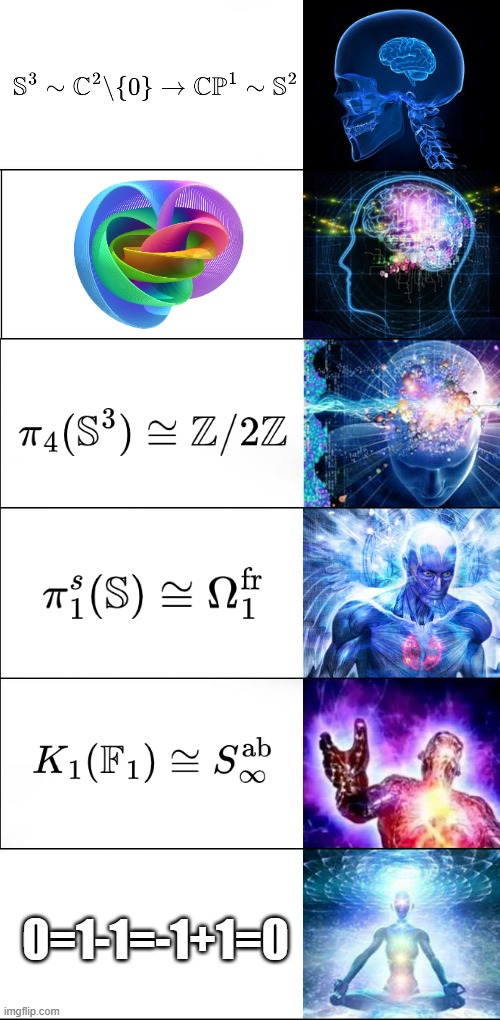
\includegraphics[height=0.8\textheight]{figures/hopf_meme.jpg}
  \end{center}
\end{figure}

\end{frame}

\section{Topology}


\begin{frame}{Hopf fibration}

  Hopf fibration is a map defined by 

  \[ H: \mathbb{S}^3 \subset \mathbb{C}^2-\{0\} \to \mathbb{CP}^1 \cong \mathbb{S}^2, (z_1,z_2) \mapsto [z_1,z_2] \]

  For any point $x\in \mathbb{S}^2$, preimage $H^{-1}(x)$ is a circle $\mathbb{S}^1$. 
\pause
  We can visualize this map by considering $ H: \mathbb{R}^3\cong \mathbb{S}^3-\{\infty\} \to \mathbb{S}^2 $ :
\begin{figure}
  \begin{center}
    \href{https://www.youtube.com/watch?v=AKotMPGFJYk}{ 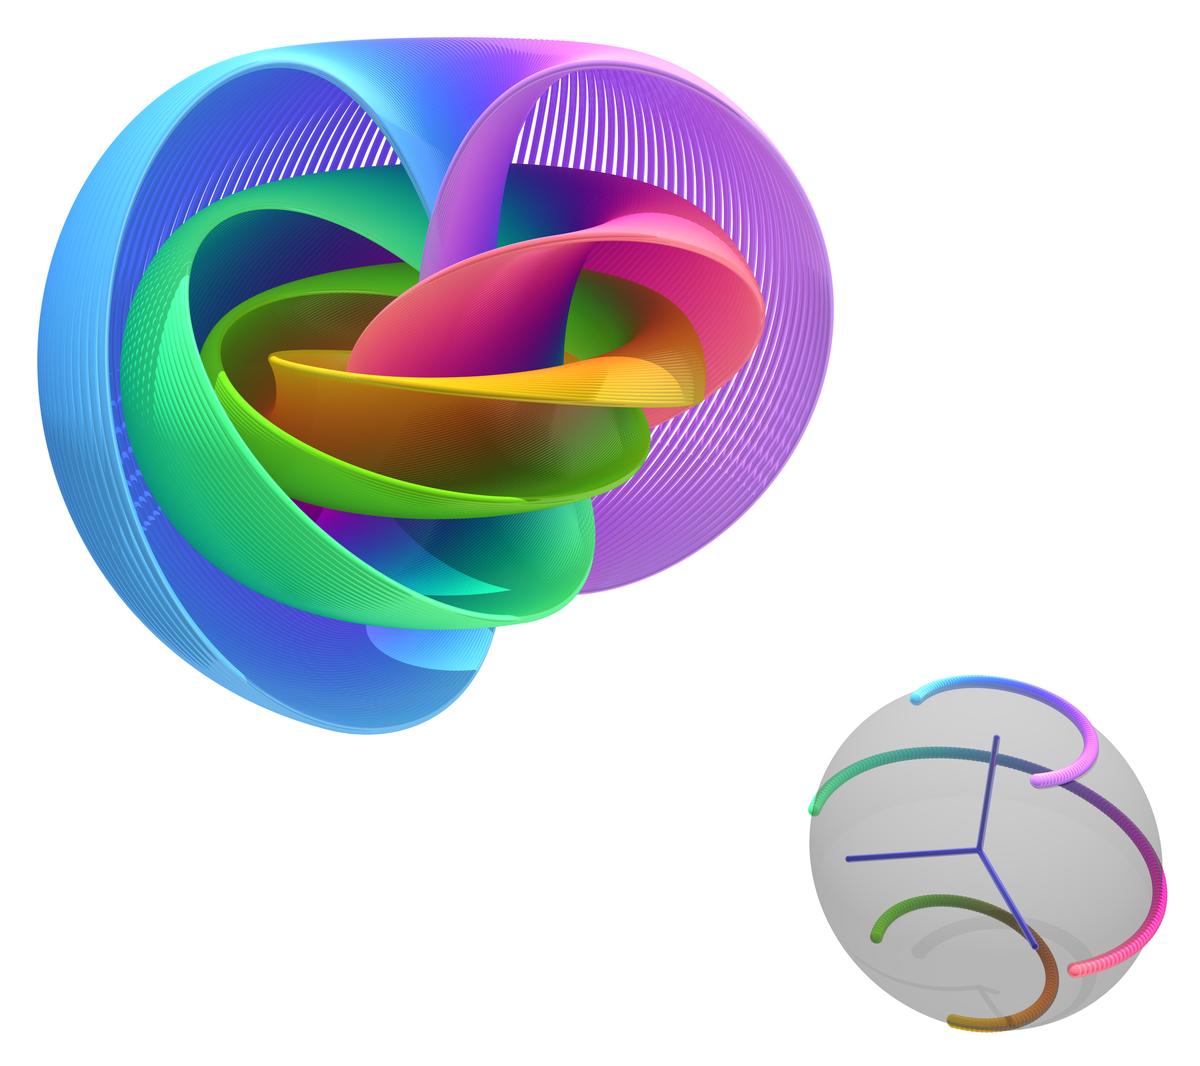
\includegraphics[height= 0.4\textheight]{figures/Hopf_Fibration.png} }
  \end{center}
\end{figure}

\end{frame}

\begin{frame}{Homotopy groups}
To understand a space $X$, we use some homotopy invariants:
\pause
\begin{itemize}
  \item $\pi_0 X \in \mathrm{Set} $, connected component, how many "pieces" $X$ has. 
    \pause
  \item Chose a base point $x\in X$, Let $ \mathrm{Map}_*(\mathbb{S}^1,X)  \in \mathrm{Space}$ be the space of loops in $X$ started from $x$. Here $\mathrm{Map}_*$ is the space of pointed continue maps, the continue structure comes from deform maps. 
    \pause
  \item $ \pi_1(X,x) := \pi_0\mathrm{Map}_*(\mathbb{S}^1,X) \in \mathrm{Group}$, how many loops in $X$ up to deformation. This is fundamental group.
    \pause
  \item $i>1, \pi_i(X,x) := \pi_0\mathrm{Map}_*(\mathbb{S}^i,X)\cong \pi_0\mathrm{Map}_*(\mathbb{S}^1,\mathrm{Map}_*(\mathbb{S}^{i-1},X)) \in \mathrm{Abel}$. This is homotopy group.
\end{itemize}
\pause
Let us study the cases $X=\mathbb{S}^n$.
\end{frame}

\begin{frame}<1-3>[label=ldm]{Homotopy groups of spheres}
\begin{itemize}
  \item For $i<n$, $\pi_i(\mathbb{S}^n)=\{ 0 \}$, where $0: \mathbb{S}^i\to * \xrightarrow{\mathrm{base}} \mathbb{S}^n$.
    \pause
  \item For $\pi_n(\mathbb{S}^n)$, let's consider the space $\mathrm{End}_*(\mathbb{S}^n):=\mathrm{Map}_*(\mathbb{S}^n,\mathbb{S}^n)$.
\end{itemize}
\pause

Let $f\in \mathrm{End}_*(\mathbb{S}^n)$, take a small disk $D^n_{\epsilon}\subset \mathbb{S}^n$ away from the base point. Then the preimage $f^{-1}(D^n_{\epsilon})\subset \mathbb{S}^n-\{*\}\cong \mathbb{R}^n$ is a disjoint union of disks for $\epsilon$ small enough. Notice that the disks in the union have orientations $+$ and $-$.

\only<4>{
\begin{center}
  

\tikzset{every picture/.style={line width=0.75pt}} %set default line width to 0.75pt        

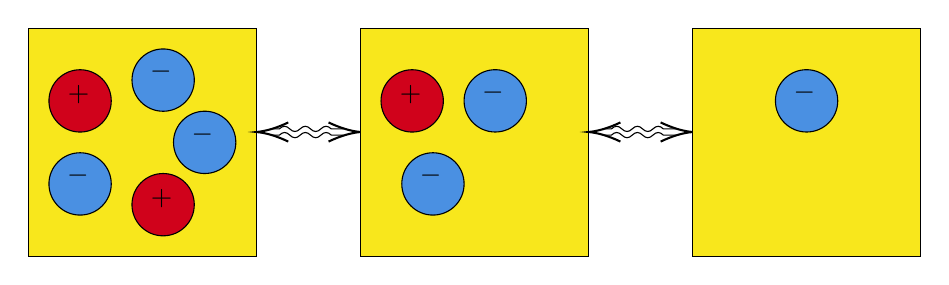
\begin{tikzpicture}[x=0.75pt,y=0.75pt,yscale=-1,xscale=1]
%uncomment if require: \path (0,202); %set diagram left start at 0, and has height of 202

%Shape: Square [id:dp8905246913749407] 
\draw  [fill={rgb, 255:red, 248; green, 231; blue, 28 }  ,fill opacity=1 ] (20,30) -- (130,30) -- (130,140) -- (20,140) -- cycle ;
%Shape: Ellipse [id:dp4923647235979962] 
\draw  [fill={rgb, 255:red, 208; green, 2; blue, 27 }  ,fill opacity=1 ] (29.98,65.01) .. controls (29.98,56.72) and (36.7,50) .. (44.99,50) .. controls (53.28,50) and (60,56.72) .. (60,65.01) .. controls (60,73.3) and (53.28,80.02) .. (44.99,80.02) .. controls (36.7,80.02) and (29.98,73.3) .. (29.98,65.01) -- cycle ;

%Shape: Ellipse [id:dp34722992258516694] 
\draw  [fill={rgb, 255:red, 74; green, 144; blue, 226 }  ,fill opacity=1 ] (29.98,105.01) .. controls (29.98,96.72) and (36.7,90) .. (44.99,90) .. controls (53.28,90) and (60,96.72) .. (60,105.01) .. controls (60,113.3) and (53.28,120.02) .. (44.99,120.02) .. controls (36.7,120.02) and (29.98,113.3) .. (29.98,105.01) -- cycle ;

%Shape: Ellipse [id:dp27578992636850996] 
\draw  [fill={rgb, 255:red, 74; green, 144; blue, 226 }  ,fill opacity=1 ] (70,54.99) .. controls (70,46.7) and (76.72,39.98) .. (85.01,39.98) .. controls (93.3,39.98) and (100.02,46.7) .. (100.02,54.99) .. controls (100.02,63.28) and (93.3,70) .. (85.01,70) .. controls (76.72,70) and (70,63.28) .. (70,54.99) -- cycle ;

%Shape: Ellipse [id:dp28012353680678137] 
\draw  [fill={rgb, 255:red, 208; green, 2; blue, 27 }  ,fill opacity=1 ] (69.98,115.01) .. controls (69.98,106.72) and (76.7,100) .. (84.99,100) .. controls (93.28,100) and (100,106.72) .. (100,115.01) .. controls (100,123.3) and (93.28,130.02) .. (84.99,130.02) .. controls (76.7,130.02) and (69.98,123.3) .. (69.98,115.01) -- cycle ;

%Shape: Ellipse [id:dp720738770484213] 
\draw  [fill={rgb, 255:red, 74; green, 144; blue, 226 }  ,fill opacity=1 ] (90,84.99) .. controls (90,76.7) and (96.72,69.98) .. (105.01,69.98) .. controls (113.3,69.98) and (120.02,76.7) .. (120.02,84.99) .. controls (120.02,93.28) and (113.3,100) .. (105.01,100) .. controls (96.72,100) and (90,93.28) .. (90,84.99) -- cycle ;

%Straight Lines [id:da3463089522780478] 
\draw    (138,78.5) -- (141,78.5) .. controls (142.67,76.83) and (144.33,76.83) .. (146,78.5) .. controls (147.67,80.17) and (149.33,80.17) .. (151,78.5) .. controls (152.67,76.83) and (154.33,76.83) .. (156,78.5) .. controls (157.67,80.17) and (159.33,80.17) .. (161,78.5) .. controls (162.67,76.83) and (164.33,76.83) .. (166,78.5) -- (169,78.5) -- (172,78.5)(138,81.5) -- (141,81.5) .. controls (142.67,79.83) and (144.33,79.83) .. (146,81.5) .. controls (147.67,83.17) and (149.33,83.17) .. (151,81.5) .. controls (152.67,79.83) and (154.33,79.83) .. (156,81.5) .. controls (157.67,83.17) and (159.33,83.17) .. (161,81.5) .. controls (162.67,79.83) and (164.33,79.83) .. (166,81.5) -- (169,81.5) -- (172,81.5) ;
\draw [shift={(180,80)}, rotate = 180] [color={rgb, 255:red, 0; green, 0; blue, 0 }  ][line width=0.75]    (15.3,-4.61) .. controls (9.73,-1.96) and (4.63,-0.42) .. (0,0) .. controls (4.63,0.42) and (9.73,1.96) .. (15.3,4.61)   ;
\draw [shift={(130,80)}, rotate = 0] [color={rgb, 255:red, 0; green, 0; blue, 0 }  ][line width=0.75]    (15.3,-4.61) .. controls (9.73,-1.96) and (4.63,-0.42) .. (0,0) .. controls (4.63,0.42) and (9.73,1.96) .. (15.3,4.61)   ;
%Shape: Square [id:dp7083023491538014] 
\draw  [fill={rgb, 255:red, 248; green, 231; blue, 28 }  ,fill opacity=1 ] (180,30) -- (290,30) -- (290,140) -- (180,140) -- cycle ;
%Shape: Ellipse [id:dp5927711612585445] 
\draw  [fill={rgb, 255:red, 208; green, 2; blue, 27 }  ,fill opacity=1 ] (189.98,65.01) .. controls (189.98,56.72) and (196.7,50) .. (204.99,50) .. controls (213.28,50) and (220,56.72) .. (220,65.01) .. controls (220,73.3) and (213.28,80.02) .. (204.99,80.02) .. controls (196.7,80.02) and (189.98,73.3) .. (189.98,65.01) -- cycle ;

%Shape: Ellipse [id:dp8226989422743765] 
\draw  [fill={rgb, 255:red, 74; green, 144; blue, 226 }  ,fill opacity=1 ] (199.98,105.01) .. controls (199.98,96.72) and (206.7,90) .. (214.99,90) .. controls (223.28,90) and (230,96.72) .. (230,105.01) .. controls (230,113.3) and (223.28,120.02) .. (214.99,120.02) .. controls (206.7,120.02) and (199.98,113.3) .. (199.98,105.01) -- cycle ;

%Shape: Ellipse [id:dp29490845567419943] 
\draw  [fill={rgb, 255:red, 74; green, 144; blue, 226 }  ,fill opacity=1 ] (230,64.99) .. controls (230,56.7) and (236.72,49.98) .. (245.01,49.98) .. controls (253.3,49.98) and (260.02,56.7) .. (260.02,64.99) .. controls (260.02,73.28) and (253.3,80) .. (245.01,80) .. controls (236.72,80) and (230,73.28) .. (230,64.99) -- cycle ;

%Straight Lines [id:da08693758592549328] 
\draw    (298,78.5) -- (301,78.5) .. controls (302.67,76.83) and (304.33,76.83) .. (306,78.5) .. controls (307.67,80.17) and (309.33,80.17) .. (311,78.5) .. controls (312.67,76.83) and (314.33,76.83) .. (316,78.5) .. controls (317.67,80.17) and (319.33,80.17) .. (321,78.5) .. controls (322.67,76.83) and (324.33,76.83) .. (326,78.5) -- (329,78.5) -- (332,78.5)(298,81.5) -- (301,81.5) .. controls (302.67,79.83) and (304.33,79.83) .. (306,81.5) .. controls (307.67,83.17) and (309.33,83.17) .. (311,81.5) .. controls (312.67,79.83) and (314.33,79.83) .. (316,81.5) .. controls (317.67,83.17) and (319.33,83.17) .. (321,81.5) .. controls (322.67,79.83) and (324.33,79.83) .. (326,81.5) -- (329,81.5) -- (332,81.5) ;
\draw [shift={(340,80)}, rotate = 180] [color={rgb, 255:red, 0; green, 0; blue, 0 }  ][line width=0.75]    (15.3,-4.61) .. controls (9.73,-1.96) and (4.63,-0.42) .. (0,0) .. controls (4.63,0.42) and (9.73,1.96) .. (15.3,4.61)   ;
\draw [shift={(290,80)}, rotate = 0] [color={rgb, 255:red, 0; green, 0; blue, 0 }  ][line width=0.75]    (15.3,-4.61) .. controls (9.73,-1.96) and (4.63,-0.42) .. (0,0) .. controls (4.63,0.42) and (9.73,1.96) .. (15.3,4.61)   ;
%Shape: Square [id:dp3405215676117721] 
\draw  [fill={rgb, 255:red, 248; green, 231; blue, 28 }  ,fill opacity=1 ] (340,30) -- (450,30) -- (450,140) -- (340,140) -- cycle ;
%Shape: Ellipse [id:dp1508940159235368] 
\draw  [fill={rgb, 255:red, 74; green, 144; blue, 226 }  ,fill opacity=1 ] (380,64.99) .. controls (380,56.7) and (386.72,49.98) .. (395.01,49.98) .. controls (403.3,49.98) and (410.02,56.7) .. (410.02,64.99) .. controls (410.02,73.28) and (403.3,80) .. (395.01,80) .. controls (386.72,80) and (380,73.28) .. (380,64.99) -- cycle ;


% Text Node
\draw (77.81,106.21) node [anchor=north west][inner sep=0.75pt]    {$+$};
% Text Node
\draw (77.46,45.32) node [anchor=north west][inner sep=0.75pt]    {$-$};
% Text Node
\draw (37.44,95.34) node [anchor=north west][inner sep=0.75pt]    {$-$};
% Text Node
\draw (37.81,56.21) node [anchor=north west][inner sep=0.75pt]    {$+$};
% Text Node
\draw (97.46,75.32) node [anchor=north west][inner sep=0.75pt]    {$-$};
% Text Node
\draw (237.46,55.32) node [anchor=north west][inner sep=0.75pt]    {$-$};
% Text Node
\draw (207.44,95.34) node [anchor=north west][inner sep=0.75pt]    {$-$};
% Text Node
\draw (197.81,56.21) node [anchor=north west][inner sep=0.75pt]    {$+$};
% Text Node
\draw (387.46,55.32) node [anchor=north west][inner sep=0.75pt]    {$-$};


\end{tikzpicture}
\end{center}
}
\only<5>{
This gives an isomorphism to the configuration space of disks. 
\[ \mathrm{End}_*(\mathbb{S}^n) \cong \mathrm{Conf}^{fr}( \mathbb{R}^n) = \bigcup_{j,k}\mathrm{Emb}( \bigsqcup_j D^n_+ \sqcup \bigsqcup_k D^n_- , \mathbb{R}^n )
\]
Therefore, $\pi_0 \mathrm{End}_*(\mathbb{S}^n) \cong \mathbb{Z}, (j,k) \mapsto j-k$
}
\end{frame}

\begin{frame}

\begin{center}
  


\tikzset{every picture/.style={line width=0.75pt}} %set default line width to 0.75pt        

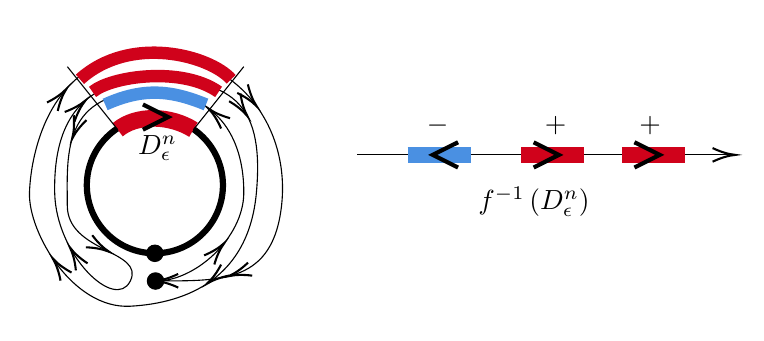
\begin{tikzpicture}[x=0.75pt,y=0.75pt,yscale=-1,xscale=1]
%uncomment if require: \path (0,153); %set diagram left start at 0, and has height of 153

%Straight Lines [id:da9147837729834951] 
\draw    (207.84,58.14) -- (388,58.14) ;
\draw [shift={(390,58.14)}, rotate = 180] [color={rgb, 255:red, 0; green, 0; blue, 0 }  ][line width=0.75]    (10.93,-3.29) .. controls (6.95,-1.4) and (3.31,-0.3) .. (0,0) .. controls (3.31,0.3) and (6.95,1.4) .. (10.93,3.29)   ;
%Shape: Circle [id:dp5777531688919217] 
\draw  [color={rgb, 255:red, 0; green, 0; blue, 0 }  ,draw opacity=1 ][line width=2.25]  (77.57,72.76) .. controls (77.57,54.65) and (92.25,39.97) .. (110.36,39.97) .. controls (128.47,39.97) and (143.15,54.65) .. (143.15,72.76) .. controls (143.15,90.87) and (128.47,105.55) .. (110.36,105.55) .. controls (92.25,105.55) and (77.57,90.87) .. (77.57,72.76) -- cycle ;
%Shape: Ellipse [id:dp9102995156755569] 
\draw  [fill={rgb, 255:red, 0; green, 0; blue, 0 }  ,fill opacity=1 ] (106.41,105.55) .. controls (106.41,103.37) and (108.18,101.6) .. (110.36,101.6) .. controls (112.54,101.6) and (114.31,103.37) .. (114.31,105.55) .. controls (114.31,107.73) and (112.54,109.49) .. (110.36,109.49) .. controls (108.18,109.49) and (106.41,107.73) .. (106.41,105.55) -- cycle ;
%Curve Lines [id:da5228835129809426] 
\draw    (110.66,118.9) .. controls (129.49,119.21) and (153.1,98.22) .. (153.2,76.36) .. controls (153.29,54.5) and (144.12,26.23) .. (104.62,27.79) .. controls (65.12,29.34) and (68.16,59.7) .. (68.16,82.47) .. controls (68.16,105.24) and (105.79,104.06) .. (98.52,118.9) .. controls (91.25,133.75) and (62.7,106.46) .. (62.09,76.4) .. controls (61.48,46.34) and (71.83,21.41) .. (110.69,21.71) .. controls (149.55,22.02) and (162.96,35.39) .. (159.27,76.36) .. controls (155.57,117.33) and (126.22,129.55) .. (98.52,131.05) .. controls (70.82,132.55) and (49.34,95.53) .. (49.94,76.4) .. controls (50.55,57.27) and (59.69,11.09) .. (104.62,9.57) .. controls (149.55,8.05) and (175.66,43.88) .. (171.41,82.43) .. controls (167.25,120.22) and (142.06,118.68) .. (112.48,118.89) ;
\draw [shift={(110.66,118.9)}, rotate = 359.43] [color={rgb, 255:red, 0; green, 0; blue, 0 }  ][line width=0.75]    (10.93,-3.29) .. controls (6.95,-1.4) and (3.31,-0.3) .. (0,0) .. controls (3.31,0.3) and (6.95,1.4) .. (10.93,3.29)   ;
\draw [shift={(143.82,100.6)}, rotate = 131.76] [color={rgb, 255:red, 0; green, 0; blue, 0 }  ][line width=0.75]    (10.93,-3.29) .. controls (6.95,-1.4) and (3.31,-0.3) .. (0,0) .. controls (3.31,0.3) and (6.95,1.4) .. (10.93,3.29)   ;
\draw [shift={(136.16,35.78)}, rotate = 40.93] [color={rgb, 255:red, 0; green, 0; blue, 0 }  ][line width=0.75]    (10.93,-3.29) .. controls (6.95,-1.4) and (3.31,-0.3) .. (0,0) .. controls (3.31,0.3) and (6.95,1.4) .. (10.93,3.29)   ;
\draw [shift={(70.47,50.44)}, rotate = 290.71] [color={rgb, 255:red, 0; green, 0; blue, 0 }  ][line width=0.75]    (10.93,-3.29) .. controls (6.95,-1.4) and (3.31,-0.3) .. (0,0) .. controls (3.31,0.3) and (6.95,1.4) .. (10.93,3.29)   ;
\draw [shift={(88.33,104.83)}, rotate = 207.7] [color={rgb, 255:red, 0; green, 0; blue, 0 }  ][line width=0.75]    (10.93,-3.29) .. controls (6.95,-1.4) and (3.31,-0.3) .. (0,0) .. controls (3.31,0.3) and (6.95,1.4) .. (10.93,3.29)   ;
\draw [shift={(69.44,102.75)}, rotate = 58.77] [color={rgb, 255:red, 0; green, 0; blue, 0 }  ][line width=0.75]    (10.93,-3.29) .. controls (6.95,-1.4) and (3.31,-0.3) .. (0,0) .. controls (3.31,0.3) and (6.95,1.4) .. (10.93,3.29)   ;
\draw [shift={(76.91,31.93)}, rotate = 134.27] [color={rgb, 255:red, 0; green, 0; blue, 0 }  ][line width=0.75]    (10.93,-3.29) .. controls (6.95,-1.4) and (3.31,-0.3) .. (0,0) .. controls (3.31,0.3) and (6.95,1.4) .. (10.93,3.29)   ;
\draw [shift={(154.96,39.51)}, rotate = 236.01] [color={rgb, 255:red, 0; green, 0; blue, 0 }  ][line width=0.75]    (10.93,-3.29) .. controls (6.95,-1.4) and (3.31,-0.3) .. (0,0) .. controls (3.31,0.3) and (6.95,1.4) .. (10.93,3.29)   ;
\draw [shift={(135.49,120.19)}, rotate = 323.14] [color={rgb, 255:red, 0; green, 0; blue, 0 }  ][line width=0.75]    (10.93,-3.29) .. controls (6.95,-1.4) and (3.31,-0.3) .. (0,0) .. controls (3.31,0.3) and (6.95,1.4) .. (10.93,3.29)   ;
\draw [shift={(61.1,107.95)}, rotate = 53.8] [color={rgb, 255:red, 0; green, 0; blue, 0 }  ][line width=0.75]    (10.93,-3.29) .. controls (6.95,-1.4) and (3.31,-0.3) .. (0,0) .. controls (3.31,0.3) and (6.95,1.4) .. (10.93,3.29)   ;
\draw [shift={(67.74,26.34)}, rotate = 128.24] [color={rgb, 255:red, 0; green, 0; blue, 0 }  ][line width=0.75]    (10.93,-3.29) .. controls (6.95,-1.4) and (3.31,-0.3) .. (0,0) .. controls (3.31,0.3) and (6.95,1.4) .. (10.93,3.29)   ;
\draw [shift={(159.44,34.76)}, rotate = 231.25] [color={rgb, 255:red, 0; green, 0; blue, 0 }  ][line width=0.75]    (10.93,-3.29) .. controls (6.95,-1.4) and (3.31,-0.3) .. (0,0) .. controls (3.31,0.3) and (6.95,1.4) .. (10.93,3.29)   ;
\draw [shift={(145.85,116.6)}, rotate = 341.86] [color={rgb, 255:red, 0; green, 0; blue, 0 }  ][line width=0.75]    (10.93,-3.29) .. controls (6.95,-1.4) and (3.31,-0.3) .. (0,0) .. controls (3.31,0.3) and (6.95,1.4) .. (10.93,3.29)   ;
%Shape: Circle [id:dp4888414439096558] 
\draw  [fill={rgb, 255:red, 0; green, 0; blue, 0 }  ,fill opacity=1 ] (106.72,118.9) .. controls (106.72,116.72) and (108.48,114.96) .. (110.66,114.96) .. controls (112.84,114.96) and (114.61,116.72) .. (114.61,118.9) .. controls (114.61,121.08) and (112.84,122.85) .. (110.66,122.85) .. controls (108.48,122.85) and (106.72,121.08) .. (106.72,118.9) -- cycle ;
%Curve Lines [id:da5649743485651755] 
\draw [color={rgb, 255:red, 208; green, 2; blue, 27 }  ,draw opacity=1 ][line width=6]    (92.48,46) .. controls (101.58,38.41) and (117.98,39.02) .. (128.91,46) ;
\draw  [color={rgb, 255:red, 0; green, 0; blue, 0 }  ,draw opacity=1 ][line width=1.5]  (104.62,33.86) -- (116.76,39.93) -- (104.62,46) ;
%Straight Lines [id:da12144641678689427] 
\draw    (68.19,15.64) -- (92.48,46) ;
%Straight Lines [id:da8252449195319262] 
\draw    (153.2,15.64) -- (128.91,46) ;
%Curve Lines [id:da15764960627001368] 
\draw [color={rgb, 255:red, 74; green, 144; blue, 226 }  ,draw opacity=1 ][line width=4.5]    (86.4,33.86) .. controls (104.62,25.66) and (117.98,26.87) .. (134.98,33.86) ;
%Curve Lines [id:da9785093166318308] 
\draw [color={rgb, 255:red, 208; green, 2; blue, 27 }  ,draw opacity=1 ][line width=4.5]    (80.33,27.79) .. controls (89.44,20.2) and (123.44,15.34) .. (141.05,27.79) ;
%Curve Lines [id:da07355354472310083] 
\draw [color={rgb, 255:red, 208; green, 2; blue, 27 }  ,draw opacity=1 ][line width=4.5]    (74.26,21.71) .. controls (98.55,-0.15) and (136.8,10.18) .. (147.12,21.71) ;
%Straight Lines [id:da7371503012271712] 
\draw [color={rgb, 255:red, 74; green, 144; blue, 226 }  ,draw opacity=1 ][line width=6]    (232.13,58.14) -- (262.49,58.14) ;
%Straight Lines [id:da0624911475429073] 
\draw [color={rgb, 255:red, 208; green, 2; blue, 27 }  ,draw opacity=1 ][line width=6]    (286.78,58.14) -- (317.14,58.14) ;
%Straight Lines [id:da9018444081119195] 
\draw [color={rgb, 255:red, 208; green, 2; blue, 27 }  ,draw opacity=1 ][line width=6]    (335.35,58.14) -- (365.71,58.14) ;
\draw  [color={rgb, 255:red, 0; green, 0; blue, 0 }  ,draw opacity=1 ][line width=1.5]  (292.85,52.07) -- (304.99,58.14) -- (292.85,64.22) ;
\draw  [color={rgb, 255:red, 0; green, 0; blue, 0 }  ,draw opacity=1 ][line width=1.5]  (341.42,52.07) -- (353.57,58.14) -- (341.42,64.22) ;
\draw  [color={rgb, 255:red, 0; green, 0; blue, 0 }  ,draw opacity=1 ][line width=1.5]  (256.42,64.22) -- (244.27,58.14) -- (256.42,52.07) ;

% Text Node
\draw (101,47.4) node [anchor=north west][inner sep=0.75pt]    {$D_{\epsilon }^{n}$};
% Text Node
\draw (265,72.4) node [anchor=north west][inner sep=0.75pt]    {$f^{-1}\left( D_{\epsilon }^{n}\right)$};
% Text Node
\draw (240.1,38.4) node [anchor=north west][inner sep=0.75pt]    {$-$};
% Text Node
\draw (296.98,38.4) node [anchor=north west][inner sep=0.75pt]    {$+$};
% Text Node
\draw (342.51,38.4) node [anchor=north west][inner sep=0.75pt]    {$+$};


\end{tikzpicture}

\pause


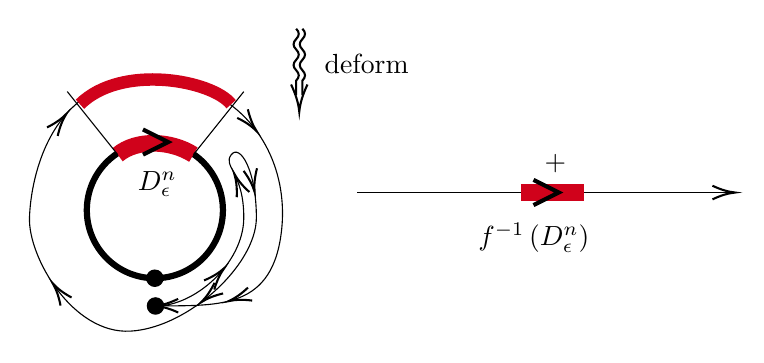
\begin{tikzpicture}[x=0.75pt,y=0.75pt,yscale=-1,xscale=1]
%uncomment if require: \path (0,167); %set diagram left start at 0, and has height of 167

%Straight Lines [id:da4097109424678873] 
\draw    (207.86,78.93) -- (388,78.93) ;
\draw [shift={(390,78.93)}, rotate = 180] [color={rgb, 255:red, 0; green, 0; blue, 0 }  ][line width=0.75]    (10.93,-3.29) .. controls (6.95,-1.4) and (3.31,-0.3) .. (0,0) .. controls (3.31,0.3) and (6.95,1.4) .. (10.93,3.29)   ;
%Shape: Ellipse [id:dp2037933356114996] 
\draw  [color={rgb, 255:red, 0; green, 0; blue, 0 }  ,draw opacity=1 ][line width=2.25]  (77.64,87.43) .. controls (77.64,69.32) and (92.32,54.64) .. (110.42,54.64) .. controls (128.53,54.64) and (143.21,69.32) .. (143.21,87.43) .. controls (143.21,105.54) and (128.53,120.21) .. (110.42,120.21) .. controls (92.32,120.21) and (77.64,105.54) .. (77.64,87.43) -- cycle ;
%Shape: Circle [id:dp21985344798556072] 
\draw  [fill={rgb, 255:red, 0; green, 0; blue, 0 }  ,fill opacity=1 ] (106.48,120.21) .. controls (106.48,118.03) and (108.24,116.27) .. (110.42,116.27) .. controls (112.6,116.27) and (114.37,118.03) .. (114.37,120.21) .. controls (114.37,122.39) and (112.6,124.16) .. (110.42,124.16) .. controls (108.24,124.16) and (106.48,122.39) .. (106.48,120.21) -- cycle ;
%Curve Lines [id:da05877208868362671] 
\draw    (110.73,133.57) .. controls (129.55,133.88) and (153.16,112.97) .. (153.26,91.12) .. controls (153.35,69.26) and (142.98,66.35) .. (147.18,60.76) .. controls (151.39,55.16) and (159.33,68.26) .. (159.33,91.03) .. controls (159.33,113.8) and (126.28,144.21) .. (98.58,145.71) .. controls (70.89,147.21) and (49.41,110.2) .. (50.01,91.07) .. controls (50.62,71.95) and (59.76,25.76) .. (104.68,24.25) .. controls (149.61,22.73) and (175.72,58.55) .. (171.47,97.1) .. controls (167.3,134.89) and (142.12,133.35) .. (112.54,133.56) ;
\draw [shift={(110.73,133.57)}, rotate = 359.43] [color={rgb, 255:red, 0; green, 0; blue, 0 }  ][line width=0.75]    (10.93,-3.29) .. controls (6.95,-1.4) and (3.31,-0.3) .. (0,0) .. controls (3.31,0.3) and (6.95,1.4) .. (10.93,3.29)   ;
\draw [shift={(143.88,115.32)}, rotate = 131.83] [color={rgb, 255:red, 0; green, 0; blue, 0 }  ][line width=0.75]    (10.93,-3.29) .. controls (6.95,-1.4) and (3.31,-0.3) .. (0,0) .. controls (3.31,0.3) and (6.95,1.4) .. (10.93,3.29)   ;
\draw [shift={(148.68,69.84)}, rotate = 67.32] [color={rgb, 255:red, 0; green, 0; blue, 0 }  ][line width=0.75]    (10.93,-3.29) .. controls (6.95,-1.4) and (3.31,-0.3) .. (0,0) .. controls (3.31,0.3) and (6.95,1.4) .. (10.93,3.29)   ;
\draw [shift={(158.47,78.6)}, rotate = 259.13] [color={rgb, 255:red, 0; green, 0; blue, 0 }  ][line width=0.75]    (10.93,-3.29) .. controls (6.95,-1.4) and (3.31,-0.3) .. (0,0) .. controls (3.31,0.3) and (6.95,1.4) .. (10.93,3.29)   ;
\draw [shift={(132.7,131.81)}, rotate = 321.34] [color={rgb, 255:red, 0; green, 0; blue, 0 }  ][line width=0.75]    (10.93,-3.29) .. controls (6.95,-1.4) and (3.31,-0.3) .. (0,0) .. controls (3.31,0.3) and (6.95,1.4) .. (10.93,3.29)   ;
\draw [shift={(61.17,122.62)}, rotate = 53.8] [color={rgb, 255:red, 0; green, 0; blue, 0 }  ][line width=0.75]    (10.93,-3.29) .. controls (6.95,-1.4) and (3.31,-0.3) .. (0,0) .. controls (3.31,0.3) and (6.95,1.4) .. (10.93,3.29)   ;
\draw [shift={(67.8,41.01)}, rotate = 128.24] [color={rgb, 255:red, 0; green, 0; blue, 0 }  ][line width=0.75]    (10.93,-3.29) .. controls (6.95,-1.4) and (3.31,-0.3) .. (0,0) .. controls (3.31,0.3) and (6.95,1.4) .. (10.93,3.29)   ;
\draw [shift={(159.5,49.43)}, rotate = 231.25] [color={rgb, 255:red, 0; green, 0; blue, 0 }  ][line width=0.75]    (10.93,-3.29) .. controls (6.95,-1.4) and (3.31,-0.3) .. (0,0) .. controls (3.31,0.3) and (6.95,1.4) .. (10.93,3.29)   ;
\draw [shift={(145.91,131.26)}, rotate = 341.86] [color={rgb, 255:red, 0; green, 0; blue, 0 }  ][line width=0.75]    (10.93,-3.29) .. controls (6.95,-1.4) and (3.31,-0.3) .. (0,0) .. controls (3.31,0.3) and (6.95,1.4) .. (10.93,3.29)   ;
%Shape: Ellipse [id:dp4119319162412425] 
\draw  [fill={rgb, 255:red, 0; green, 0; blue, 0 }  ,fill opacity=1 ] (106.78,133.57) .. controls (106.78,131.39) and (108.55,129.63) .. (110.73,129.63) .. controls (112.91,129.63) and (114.67,131.39) .. (114.67,133.57) .. controls (114.67,135.75) and (112.91,137.52) .. (110.73,137.52) .. controls (108.55,137.52) and (106.78,135.75) .. (106.78,133.57) -- cycle ;
%Curve Lines [id:da330753230875217] 
\draw [color={rgb, 255:red, 208; green, 2; blue, 27 }  ,draw opacity=1 ][line width=6]    (92.54,60.67) .. controls (101.65,53.08) and (118.04,53.69) .. (128.97,60.67) ;
\draw  [color={rgb, 255:red, 0; green, 0; blue, 0 }  ,draw opacity=1 ][line width=1.5]  (104.68,48.53) -- (116.83,54.6) -- (104.68,60.67) ;
%Straight Lines [id:da5299179660764051] 
\draw    (68.21,30.27) -- (92.54,60.67) ;
%Straight Lines [id:da7466964709549098] 
\draw    (153.26,30.32) -- (128.97,60.67) ;
%Curve Lines [id:da9724921884388225] 
\draw [color={rgb, 255:red, 208; green, 2; blue, 27 }  ,draw opacity=1 ][line width=4.5]    (74.33,36.39) .. controls (94.36,16.66) and (138.04,24.81) .. (147.18,36.39) ;
%Straight Lines [id:da26217806562722235] 
\draw [color={rgb, 255:red, 208; green, 2; blue, 27 }  ,draw opacity=1 ][line width=6]    (286.79,78.93) -- (317.14,78.93) ;
\draw  [color={rgb, 255:red, 0; green, 0; blue, 0 }  ,draw opacity=1 ][line width=1.5]  (292.86,72.86) -- (305,78.93) -- (292.86,85) ;
%Straight Lines [id:da5970011938083455] 
\draw [line width=0.75]    (181.5,0) .. controls (183.17,1.67) and (183.17,3.33) .. (181.5,5) .. controls (179.83,6.67) and (179.83,8.33) .. (181.5,10) .. controls (183.17,11.67) and (183.17,13.33) .. (181.5,15) .. controls (179.83,16.67) and (179.83,18.33) .. (181.5,20) .. controls (183.17,21.67) and (183.17,23.33) .. (181.5,25) -- (181.5,29) -- (181.5,32)(178.5,0) .. controls (180.17,1.67) and (180.17,3.33) .. (178.5,5) .. controls (176.83,6.67) and (176.83,8.33) .. (178.5,10) .. controls (180.17,11.67) and (180.17,13.33) .. (178.5,15) .. controls (176.83,16.67) and (176.83,18.33) .. (178.5,20) .. controls (180.17,21.67) and (180.17,23.33) .. (178.5,25) -- (178.5,29) -- (178.5,32) ;
\draw [shift={(180,40)}, rotate = 270] [color={rgb, 255:red, 0; green, 0; blue, 0 }  ][line width=0.75]    (13.12,-3.95) .. controls (8.34,-1.68) and (3.97,-0.36) .. (0,0) .. controls (3.97,0.36) and (8.34,1.68) .. (13.12,3.95)   ;

% Text Node
\draw (101,67.4) node [anchor=north west][inner sep=0.75pt]    {$D_{\epsilon }^{n}$};
% Text Node
\draw (265,92.4) node [anchor=north west][inner sep=0.75pt]    {$f^{-1}\left( D_{\epsilon }^{n}\right)$};
% Text Node
\draw (296.98,59.19) node [anchor=north west][inner sep=0.75pt]    {$+$};
% Text Node
\draw (191,11) node [anchor=north west][inner sep=0.75pt]   [align=left] {deform};


\end{tikzpicture}

\end{center}

\end{frame}

\againframe<4->{ldm}

\begin{frame}{Higher homotopy groups of spheres}
\begin{itemize}
  \item For $i>n$, $\pi_i(\mathbb{S}^n) = $ ?
    \pause
  \item For $i>1$, $ \pi_i(\mathbb{S}^1) =\{0\}$.
    \pause
  \item But $\pi_3(\mathbb{S}^2) = \pi_0 \mathrm{Map}_*(\mathbb{S}^3,\mathbb{S}^2) \ni H $, and $H \nsim 0 $, i.e. $H$ can not deform to $0$
\end{itemize}
How to see that?
\pause
\[
  \mathrm{Map}_*(\mathbb{S}^{n+1},\mathbb{S}^n) \cong \mathrm{Map}_*(\mathbb{S}^1,\mathrm{End}_*(\mathbb{S}^n))\to \mathrm{Map}_*([0,1],\mathrm{End}_*(\mathbb{S}^n))
\]
Then $H$ corresponds to a path (deformation or homotopy) form $0\in \mathrm{End}_*(\mathbb{S}^2)$ to $0$ itself.

\end{frame}
\begin{frame}{Visualize $H$ as deformation}
  I made an animation to visualize this deformation.
  \begin{figure}
    \begin{center}
      \href{https://www.youtube.com/watch?v=TnBWwh7I3aA}{ 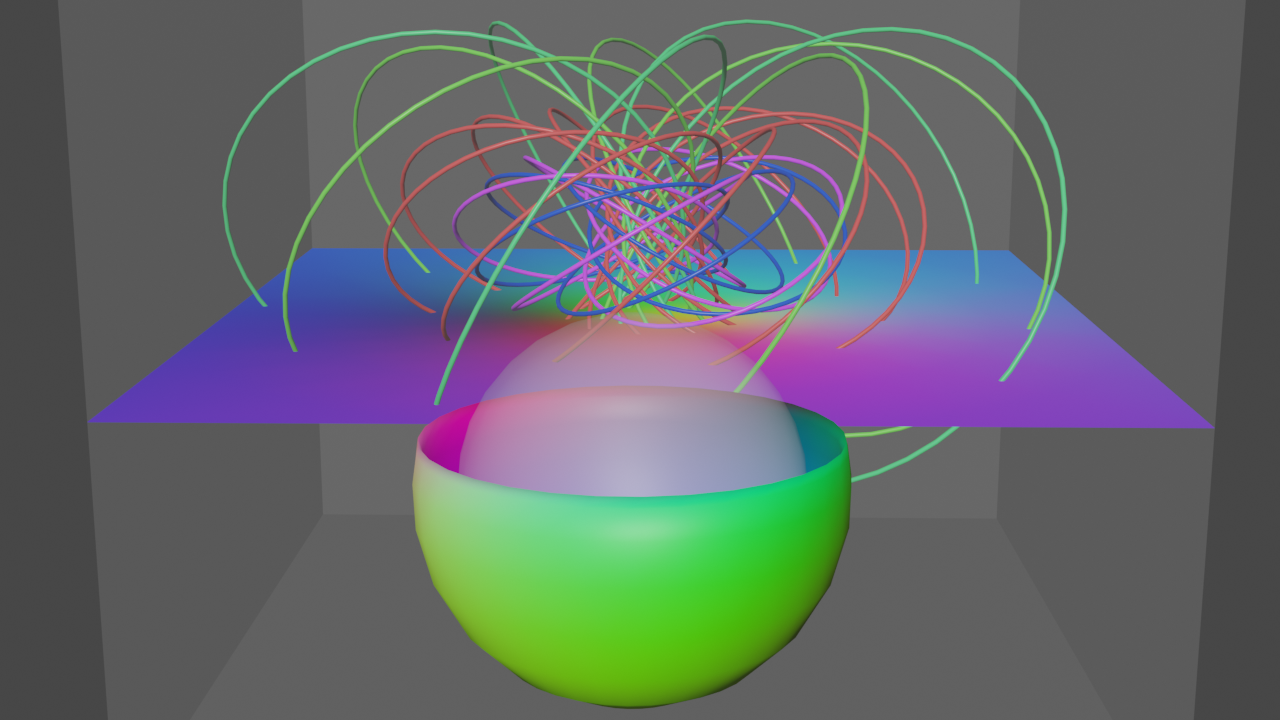
\includegraphics[height=0.3\textheight]{figures/hopf_homotopy.png} }
    \end{center}
  \end{figure}
  \pause
  We can also visualize it as a movement in the configuration space. We will show it in the end.
 


\end{frame}
\section{Algebra}

\begin{frame}{How to define $\mathbb{Z}$ ?}
\pause
We can define natural number $\mathbb{N}$ as isomorphic classes of finite sets.
\[
  \mathrm{FinSet}_{/\cong} \xrightarrow{|\cdot|} \mathbb{N}, |X \sqcup Y| = |X|+|Y| 
\]
How to define integral number $\mathbb{Z}$ with finite sets? 

\pause
We use the \textbf{Grothendieck group} $K_0(\mathrm{FinSet})$ (we can think finite set as $\mathbb{F}_1 \text{-}\mathrm{mod}$):
\[
  K_0(\mathrm{FinSet}) = \{ (X,Y)\in (\mathrm{FinSet}_{/\cong})^2   \} / \{ (X \sqcup Z , Y \sqcup Z) \sim (X,Y)\}
\]
We can think we formally define $"X-Y"$ in this way.

\pause
But what is $K_i(\mathrm{FinSet})$ for $i>0$ ?
\end{frame}
\begin{frame}{Space of "finite sets"}
  Instead of thinking the set of "finite sets", we now consider the space of them $F = \mathrm{FinSet}^{\cong}$ : every point $x\in F$ corresponds to a finite set, and a path between to points corresponds to an isomorphism $f:x\to y$ of two finite sets. 
  \pause

\begin{center}

\tikzset{every picture/.style={line width=0.75pt}} %set default line width to 0.75pt        

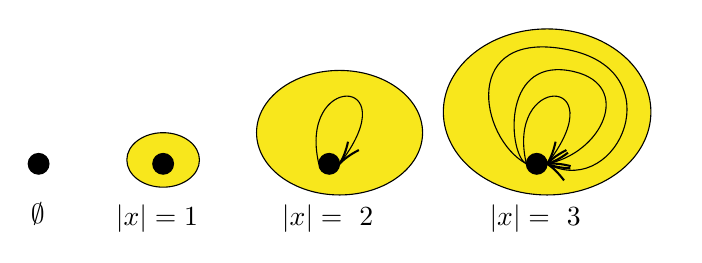
\begin{tikzpicture}[x=0.75pt,y=0.75pt,yscale=-1,xscale=1]
%uncomment if require: \path (0,157); %set diagram left start at 0, and has height of 157

%Shape: Ellipse [id:dp7720494291476914] 
\draw  [color={rgb, 255:red, 0; green, 0; blue, 0 }  ,draw opacity=1 ][fill={rgb, 255:red, 248; green, 231; blue, 28 }  ,fill opacity=1 ] (66.5,93.13) .. controls (66.5,85.88) and (74.34,80) .. (84,80) .. controls (93.66,80) and (101.5,85.88) .. (101.5,93.13) .. controls (101.5,100.37) and (93.66,106.25) .. (84,106.25) .. controls (74.34,106.25) and (66.5,100.37) .. (66.5,93.13) -- cycle ;
%Shape: Circle [id:dp8806999895439951] 
\draw  [fill={rgb, 255:red, 0; green, 0; blue, 0 }  ,fill opacity=1 ] (19,95) .. controls (19,92.24) and (21.24,90) .. (24,90) .. controls (26.76,90) and (29,92.24) .. (29,95) .. controls (29,97.76) and (26.76,100) .. (24,100) .. controls (21.24,100) and (19,97.76) .. (19,95) -- cycle ;
%Shape: Ellipse [id:dp6858466977080211] 
\draw  [color={rgb, 255:red, 0; green, 0; blue, 0 }  ,draw opacity=1 ][fill={rgb, 255:red, 248; green, 231; blue, 28 }  ,fill opacity=1 ] (129,80) .. controls (129,63.43) and (146.91,50) .. (169,50) .. controls (191.09,50) and (209,63.43) .. (209,80) .. controls (209,96.57) and (191.09,110) .. (169,110) .. controls (146.91,110) and (129,96.57) .. (129,80) -- cycle ;
%Shape: Circle [id:dp07645354210878019] 
\draw  [fill={rgb, 255:red, 0; green, 0; blue, 0 }  ,fill opacity=1 ] (79,95) .. controls (79,92.24) and (81.24,90) .. (84,90) .. controls (86.76,90) and (89,92.24) .. (89,95) .. controls (89,97.76) and (86.76,100) .. (84,100) .. controls (81.24,100) and (79,97.76) .. (79,95) -- cycle ;
%Shape: Circle [id:dp40236958016433766] 
\draw  [fill={rgb, 255:red, 0; green, 0; blue, 0 }  ,fill opacity=1 ] (159,95) .. controls (159,92.24) and (161.24,90) .. (164,90) .. controls (166.76,90) and (169,92.24) .. (169,95) .. controls (169,97.76) and (166.76,100) .. (164,100) .. controls (161.24,100) and (159,97.76) .. (159,95) -- cycle ;
%Curve Lines [id:da9320937793451245] 
\draw    (159,95) .. controls (148.85,51.44) and (201.19,51.98) .. (169.97,93.72) ;
\draw [shift={(169,95)}, rotate = 307.71] [color={rgb, 255:red, 0; green, 0; blue, 0 }  ][line width=0.75]    (10.93,-3.29) .. controls (6.95,-1.4) and (3.31,-0.3) .. (0,0) .. controls (3.31,0.3) and (6.95,1.4) .. (10.93,3.29)   ;
%Shape: Ellipse [id:dp7438442927969897] 
\draw  [color={rgb, 255:red, 0; green, 0; blue, 0 }  ,draw opacity=1 ][fill={rgb, 255:red, 248; green, 231; blue, 28 }  ,fill opacity=1 ] (219,70) .. controls (219,47.91) and (241.39,30) .. (269,30) .. controls (296.61,30) and (319,47.91) .. (319,70) .. controls (319,92.09) and (296.61,110) .. (269,110) .. controls (241.39,110) and (219,92.09) .. (219,70) -- cycle ;
%Shape: Circle [id:dp35201618999350126] 
\draw  [fill={rgb, 255:red, 0; green, 0; blue, 0 }  ,fill opacity=1 ] (259,95) .. controls (259,92.24) and (261.24,90) .. (264,90) .. controls (266.76,90) and (269,92.24) .. (269,95) .. controls (269,97.76) and (266.76,100) .. (264,100) .. controls (261.24,100) and (259,97.76) .. (259,95) -- cycle ;
%Curve Lines [id:da21588442624021154] 
\draw    (259,95) .. controls (248.85,51.44) and (301.19,51.98) .. (269.97,93.72) ;
\draw [shift={(269,95)}, rotate = 307.71] [color={rgb, 255:red, 0; green, 0; blue, 0 }  ][line width=0.75]    (10.93,-3.29) .. controls (6.95,-1.4) and (3.31,-0.3) .. (0,0) .. controls (3.31,0.3) and (6.95,1.4) .. (10.93,3.29)   ;
%Curve Lines [id:da6615814730866243] 
\draw    (259,95) .. controls (250.57,90.86) and (246.67,45) .. (279,50) .. controls (310.69,54.9) and (297.31,88.13) .. (270.65,94.64) ;
\draw [shift={(269,95)}, rotate = 348.79] [color={rgb, 255:red, 0; green, 0; blue, 0 }  ][line width=0.75]    (10.93,-3.29) .. controls (6.95,-1.4) and (3.31,-0.3) .. (0,0) .. controls (3.31,0.3) and (6.95,1.4) .. (10.93,3.29)   ;
%Curve Lines [id:da1913182351607403] 
\draw    (259,95) .. controls (236,82.33) and (227.33,29.67) .. (279,40) .. controls (329.89,50.18) and (303.49,110.81) .. (270.51,95.74) ;
\draw [shift={(269,95)}, rotate = 27.69] [color={rgb, 255:red, 0; green, 0; blue, 0 }  ][line width=0.75]    (10.93,-3.29) .. controls (6.95,-1.4) and (3.31,-0.3) .. (0,0) .. controls (3.31,0.3) and (6.95,1.4) .. (10.93,3.29)   ;

% Text Node
\draw (19,112.4) node [anchor=north west][inner sep=0.75pt]    {$\emptyset \ $};
% Text Node
\draw (60,113.4) node [anchor=north west][inner sep=0.75pt]    {$|x|=1$};
% Text Node
\draw (140,113.4) node [anchor=north west][inner sep=0.75pt]    {$|x|=\ 2$};
% Text Node
\draw (240,113.4) node [anchor=north west][inner sep=0.75pt]    {$|x|=\ 3$};
% Text Node
\draw (323,112.4) node [anchor=north west][inner sep=0.75pt]    {$\dotsc $};


\end{tikzpicture}
\end{center}
\pause
\begin{itemize}
  \item $\pi_0(F)= \mathrm{FinSet}_{/\cong} \cong \mathbb{N} $.
  \item $\pi_1(F,x) = \mathrm{S}_{|x|}$, the permutation group. 
  \item $\pi_i(F,x) = \{0\}$ for $i>1$ (one can never deform an isomorphism of set to another). 

\end{itemize}
\end{frame}
\begin{frame}{K-space (spectrum) of "finite sets"}
  We want to add "negative" to $F$. We can consider the space $K(F)$ of (ordered) finite sets, whose elements are marked by $+$ or $-$, and we also want to identify the sets with same "value" $ \| X \| =|X_+|-|X_-| $, and these identifications will be the paths.
\pause
\begin{center}


\tikzset{every picture/.style={line width=0.75pt}} %set default line width to 0.75pt        

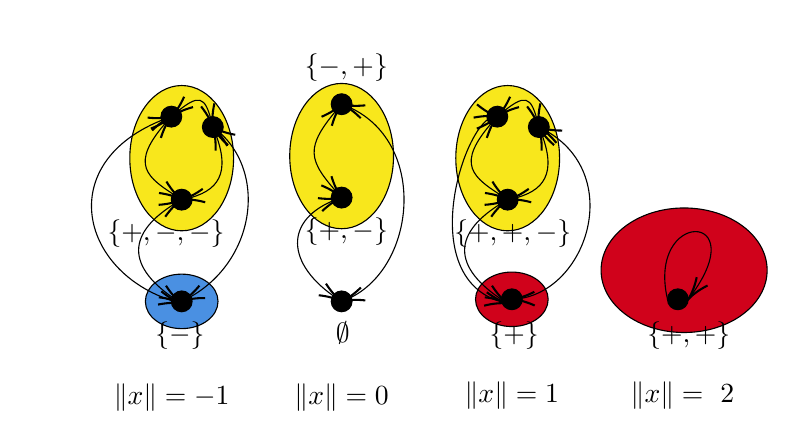
\begin{tikzpicture}[x=0.75pt,y=0.75pt,yscale=-1,xscale=1]
%uncomment if require: \path (0,243); %set diagram left start at 0, and has height of 243

%Shape: Ellipse [id:dp9584335989643185] 
\draw  [color={rgb, 255:red, 0; green, 0; blue, 0 }  ,draw opacity=1 ][fill={rgb, 255:red, 208; green, 2; blue, 27 }  ,fill opacity=1 ] (219.5,134) .. controls (219.5,126.75) and (227.34,120.88) .. (237,120.88) .. controls (246.66,120.88) and (254.5,126.75) .. (254.5,134) .. controls (254.5,141.25) and (246.66,147.13) .. (237,147.13) .. controls (227.34,147.13) and (219.5,141.25) .. (219.5,134) -- cycle ;
%Shape: Circle [id:dp6840810418640495] 
\draw  [fill={rgb, 255:red, 0; green, 0; blue, 0 }  ,fill opacity=1 ] (150,135) .. controls (150,132.24) and (152.24,130) .. (155,130) .. controls (157.76,130) and (160,132.24) .. (160,135) .. controls (160,137.76) and (157.76,140) .. (155,140) .. controls (152.24,140) and (150,137.76) .. (150,135) -- cycle ;
%Shape: Ellipse [id:dp2074209970263552] 
\draw  [color={rgb, 255:red, 0; green, 0; blue, 0 }  ,draw opacity=1 ][fill={rgb, 255:red, 208; green, 2; blue, 27 }  ,fill opacity=1 ] (280,120) .. controls (280,103.43) and (297.91,90) .. (320,90) .. controls (342.09,90) and (360,103.43) .. (360,120) .. controls (360,136.57) and (342.09,150) .. (320,150) .. controls (297.91,150) and (280,136.57) .. (280,120) -- cycle ;
%Shape: Circle [id:dp075966422192562] 
\draw  [fill={rgb, 255:red, 0; green, 0; blue, 0 }  ,fill opacity=1 ] (232,134) .. controls (232,131.24) and (234.24,129) .. (237,129) .. controls (239.76,129) and (242,131.24) .. (242,134) .. controls (242,136.76) and (239.76,139) .. (237,139) .. controls (234.24,139) and (232,136.76) .. (232,134) -- cycle ;
%Shape: Circle [id:dp13601589423138405] 
\draw  [fill={rgb, 255:red, 0; green, 0; blue, 0 }  ,fill opacity=1 ] (312,134) .. controls (312,131.24) and (314.24,129) .. (317,129) .. controls (319.76,129) and (322,131.24) .. (322,134) .. controls (322,136.76) and (319.76,139) .. (317,139) .. controls (314.24,139) and (312,136.76) .. (312,134) -- cycle ;
%Curve Lines [id:da16816986849573778] 
\draw    (312,134) .. controls (301.85,90.44) and (354.19,90.98) .. (322.97,132.72) ;
\draw [shift={(322,134)}, rotate = 307.71] [color={rgb, 255:red, 0; green, 0; blue, 0 }  ][line width=0.75]    (10.93,-3.29) .. controls (6.95,-1.4) and (3.31,-0.3) .. (0,0) .. controls (3.31,0.3) and (6.95,1.4) .. (10.93,3.29)   ;
%Shape: Ellipse [id:dp22092714462956686] 
\draw  [color={rgb, 255:red, 0; green, 0; blue, 0 }  ,draw opacity=1 ][fill={rgb, 255:red, 74; green, 144; blue, 226 }  ,fill opacity=1 ] (60.44,135) .. controls (60.44,127.75) and (68.27,121.88) .. (77.94,121.88) .. controls (87.6,121.88) and (95.44,127.75) .. (95.44,135) .. controls (95.44,142.25) and (87.6,148.13) .. (77.94,148.13) .. controls (68.27,148.13) and (60.44,142.25) .. (60.44,135) -- cycle ;
%Shape: Circle [id:dp16791708812740458] 
\draw  [fill={rgb, 255:red, 0; green, 0; blue, 0 }  ,fill opacity=1 ] (72.94,135) .. controls (72.94,132.24) and (75.18,130) .. (77.94,130) .. controls (80.7,130) and (82.94,132.24) .. (82.94,135) .. controls (82.94,137.76) and (80.7,140) .. (77.94,140) .. controls (75.18,140) and (72.94,137.76) .. (72.94,135) -- cycle ;
%Shape: Ellipse [id:dp9992132530303848] 
\draw  [color={rgb, 255:red, 0; green, 0; blue, 0 }  ,draw opacity=1 ][fill={rgb, 255:red, 248; green, 231; blue, 28 }  ,fill opacity=1 ] (130,65) .. controls (130,45.67) and (141.19,30) .. (155,30) .. controls (168.81,30) and (180,45.67) .. (180,65) .. controls (180,84.33) and (168.81,100) .. (155,100) .. controls (141.19,100) and (130,84.33) .. (130,65) -- cycle ;
%Shape: Circle [id:dp2663631471602572] 
\draw  [fill={rgb, 255:red, 0; green, 0; blue, 0 }  ,fill opacity=1 ] (150,85) .. controls (150,82.24) and (152.24,80) .. (155,80) .. controls (157.76,80) and (160,82.24) .. (160,85) .. controls (160,87.76) and (157.76,90) .. (155,90) .. controls (152.24,90) and (150,87.76) .. (150,85) -- cycle ;
%Shape: Circle [id:dp9743438242870825] 
\draw  [fill={rgb, 255:red, 0; green, 0; blue, 0 }  ,fill opacity=1 ] (150,40) .. controls (150,37.24) and (152.24,35) .. (155,35) .. controls (157.76,35) and (160,37.24) .. (160,40) .. controls (160,42.76) and (157.76,45) .. (155,45) .. controls (152.24,45) and (150,42.76) .. (150,40) -- cycle ;
%Curve Lines [id:da3723191348864274] 
\draw    (153.64,41.57) .. controls (136.87,61.11) and (138.65,66.84) .. (153.81,83.68) ;
\draw [shift={(155,85)}, rotate = 227.73] [color={rgb, 255:red, 0; green, 0; blue, 0 }  ][line width=0.75]    (10.93,-3.29) .. controls (6.95,-1.4) and (3.31,-0.3) .. (0,0) .. controls (3.31,0.3) and (6.95,1.4) .. (10.93,3.29)   ;
\draw [shift={(155,40)}, rotate = 131.19] [color={rgb, 255:red, 0; green, 0; blue, 0 }  ][line width=0.75]    (10.93,-3.29) .. controls (6.95,-1.4) and (3.31,-0.3) .. (0,0) .. controls (3.31,0.3) and (6.95,1.4) .. (10.93,3.29)   ;
%Curve Lines [id:da7917177061632026] 
\draw    (152.9,85.73) .. controls (126.91,95.3) and (127.66,117.2) .. (153.39,133.98) ;
\draw [shift={(155,135)}, rotate = 211.76] [color={rgb, 255:red, 0; green, 0; blue, 0 }  ][line width=0.75]    (10.93,-3.29) .. controls (6.95,-1.4) and (3.31,-0.3) .. (0,0) .. controls (3.31,0.3) and (6.95,1.4) .. (10.93,3.29)   ;
\draw [shift={(155,85)}, rotate = 161.97] [color={rgb, 255:red, 0; green, 0; blue, 0 }  ][line width=0.75]    (10.93,-3.29) .. controls (6.95,-1.4) and (3.31,-0.3) .. (0,0) .. controls (3.31,0.3) and (6.95,1.4) .. (10.93,3.29)   ;
%Curve Lines [id:da48696026802363557] 
\draw    (156.92,40.72) .. controls (197.51,57.08) and (191.32,120.58) .. (156.61,134.4) ;
\draw [shift={(155,135)}, rotate = 340.94] [color={rgb, 255:red, 0; green, 0; blue, 0 }  ][line width=0.75]    (10.93,-3.29) .. controls (6.95,-1.4) and (3.31,-0.3) .. (0,0) .. controls (3.31,0.3) and (6.95,1.4) .. (10.93,3.29)   ;
\draw [shift={(155,40)}, rotate = 19.49] [color={rgb, 255:red, 0; green, 0; blue, 0 }  ][line width=0.75]    (10.93,-3.29) .. controls (6.95,-1.4) and (3.31,-0.3) .. (0,0) .. controls (3.31,0.3) and (6.95,1.4) .. (10.93,3.29)   ;
%Shape: Ellipse [id:dp20966307022054598] 
\draw  [color={rgb, 255:red, 0; green, 0; blue, 0 }  ,draw opacity=1 ][fill={rgb, 255:red, 248; green, 231; blue, 28 }  ,fill opacity=1 ] (52.94,66) .. controls (52.94,46.67) and (64.13,31) .. (77.94,31) .. controls (91.74,31) and (102.94,46.67) .. (102.94,66) .. controls (102.94,85.33) and (91.74,101) .. (77.94,101) .. controls (64.13,101) and (52.94,85.33) .. (52.94,66) -- cycle ;
%Shape: Circle [id:dp9073393822290099] 
\draw  [fill={rgb, 255:red, 0; green, 0; blue, 0 }  ,fill opacity=1 ] (72.94,86) .. controls (72.94,83.24) and (75.18,81) .. (77.94,81) .. controls (80.7,81) and (82.94,83.24) .. (82.94,86) .. controls (82.94,88.76) and (80.7,91) .. (77.94,91) .. controls (75.18,91) and (72.94,88.76) .. (72.94,86) -- cycle ;
%Curve Lines [id:da9045538376069651] 
\draw    (75.94,87.15) .. controls (51.1,101.9) and (50.64,118.42) .. (76.33,134.99) ;
\draw [shift={(77.94,136)}, rotate = 211.76] [color={rgb, 255:red, 0; green, 0; blue, 0 }  ][line width=0.75]    (10.93,-3.29) .. controls (6.95,-1.4) and (3.31,-0.3) .. (0,0) .. controls (3.31,0.3) and (6.95,1.4) .. (10.93,3.29)   ;
\draw [shift={(77.94,86)}, rotate = 150.71] [color={rgb, 255:red, 0; green, 0; blue, 0 }  ][line width=0.75]    (10.93,-3.29) .. controls (6.95,-1.4) and (3.31,-0.3) .. (0,0) .. controls (3.31,0.3) and (6.95,1.4) .. (10.93,3.29)   ;
%Curve Lines [id:da022230988628577197] 
\draw    (93.76,52.98) .. controls (101.9,73.16) and (95.85,82.13) .. (79.73,85.64) ;
\draw [shift={(77.94,86)}, rotate = 349.51] [color={rgb, 255:red, 0; green, 0; blue, 0 }  ][line width=0.75]    (10.93,-3.29) .. controls (6.95,-1.4) and (3.31,-0.3) .. (0,0) .. controls (3.31,0.3) and (6.95,1.4) .. (10.93,3.29)   ;
\draw [shift={(92.94,51)}, rotate = 66.6] [color={rgb, 255:red, 0; green, 0; blue, 0 }  ][line width=0.75]    (10.93,-3.29) .. controls (6.95,-1.4) and (3.31,-0.3) .. (0,0) .. controls (3.31,0.3) and (6.95,1.4) .. (10.93,3.29)   ;
%Curve Lines [id:da2903576495179958] 
\draw    (71.32,47.77) .. controls (51.86,69.48) and (61.29,75.21) .. (76.28,84.93) ;
\draw [shift={(77.94,86)}, rotate = 213.15] [color={rgb, 255:red, 0; green, 0; blue, 0 }  ][line width=0.75]    (10.93,-3.29) .. controls (6.95,-1.4) and (3.31,-0.3) .. (0,0) .. controls (3.31,0.3) and (6.95,1.4) .. (10.93,3.29)   ;
\draw [shift={(72.94,46)}, rotate = 132.94] [color={rgb, 255:red, 0; green, 0; blue, 0 }  ][line width=0.75]    (10.93,-3.29) .. controls (6.95,-1.4) and (3.31,-0.3) .. (0,0) .. controls (3.31,0.3) and (6.95,1.4) .. (10.93,3.29)   ;
%Shape: Ellipse [id:dp036971068231425264] 
\draw  [color={rgb, 255:red, 0; green, 0; blue, 0 }  ,draw opacity=1 ][fill={rgb, 255:red, 248; green, 231; blue, 28 }  ,fill opacity=1 ] (210,66) .. controls (210,46.67) and (221.19,31) .. (235,31) .. controls (248.81,31) and (260,46.67) .. (260,66) .. controls (260,85.33) and (248.81,101) .. (235,101) .. controls (221.19,101) and (210,85.33) .. (210,66) -- cycle ;
%Shape: Circle [id:dp9059746394811838] 
\draw  [fill={rgb, 255:red, 0; green, 0; blue, 0 }  ,fill opacity=1 ] (230,86) .. controls (230,83.24) and (232.24,81) .. (235,81) .. controls (237.76,81) and (240,83.24) .. (240,86) .. controls (240,88.76) and (237.76,91) .. (235,91) .. controls (232.24,91) and (230,88.76) .. (230,86) -- cycle ;
%Curve Lines [id:da2920242121207761] 
\draw    (233,87.15) .. controls (208.16,101.9) and (207.71,118.42) .. (233.39,134.99) ;
\draw [shift={(235,136)}, rotate = 211.76] [color={rgb, 255:red, 0; green, 0; blue, 0 }  ][line width=0.75]    (10.93,-3.29) .. controls (6.95,-1.4) and (3.31,-0.3) .. (0,0) .. controls (3.31,0.3) and (6.95,1.4) .. (10.93,3.29)   ;
\draw [shift={(235,86)}, rotate = 150.71] [color={rgb, 255:red, 0; green, 0; blue, 0 }  ][line width=0.75]    (10.93,-3.29) .. controls (6.95,-1.4) and (3.31,-0.3) .. (0,0) .. controls (3.31,0.3) and (6.95,1.4) .. (10.93,3.29)   ;
%Curve Lines [id:da5347165045324522] 
\draw    (250.83,52.98) .. controls (258.96,73.16) and (252.92,82.13) .. (236.79,85.64) ;
\draw [shift={(235,86)}, rotate = 349.51] [color={rgb, 255:red, 0; green, 0; blue, 0 }  ][line width=0.75]    (10.93,-3.29) .. controls (6.95,-1.4) and (3.31,-0.3) .. (0,0) .. controls (3.31,0.3) and (6.95,1.4) .. (10.93,3.29)   ;
\draw [shift={(250,51)}, rotate = 66.6] [color={rgb, 255:red, 0; green, 0; blue, 0 }  ][line width=0.75]    (10.93,-3.29) .. controls (6.95,-1.4) and (3.31,-0.3) .. (0,0) .. controls (3.31,0.3) and (6.95,1.4) .. (10.93,3.29)   ;
%Curve Lines [id:da09527395398351857] 
\draw    (228.39,47.77) .. controls (208.93,69.48) and (218.35,75.21) .. (233.35,84.93) ;
\draw [shift={(235,86)}, rotate = 213.15] [color={rgb, 255:red, 0; green, 0; blue, 0 }  ][line width=0.75]    (10.93,-3.29) .. controls (6.95,-1.4) and (3.31,-0.3) .. (0,0) .. controls (3.31,0.3) and (6.95,1.4) .. (10.93,3.29)   ;
\draw [shift={(230,46)}, rotate = 132.94] [color={rgb, 255:red, 0; green, 0; blue, 0 }  ][line width=0.75]    (10.93,-3.29) .. controls (6.95,-1.4) and (3.31,-0.3) .. (0,0) .. controls (3.31,0.3) and (6.95,1.4) .. (10.93,3.29)   ;
%Shape: Circle [id:dp12760776343533387] 
\draw  [fill={rgb, 255:red, 0; green, 0; blue, 0 }  ,fill opacity=1 ] (67.94,46) .. controls (67.94,43.24) and (70.18,41) .. (72.94,41) .. controls (75.7,41) and (77.94,43.24) .. (77.94,46) .. controls (77.94,48.76) and (75.7,51) .. (72.94,51) .. controls (70.18,51) and (67.94,48.76) .. (67.94,46) -- cycle ;
%Shape: Circle [id:dp02366574091579099] 
\draw  [fill={rgb, 255:red, 0; green, 0; blue, 0 }  ,fill opacity=1 ] (87.94,51) .. controls (87.94,48.24) and (90.18,46) .. (92.94,46) .. controls (95.7,46) and (97.94,48.24) .. (97.94,51) .. controls (97.94,53.76) and (95.7,56) .. (92.94,56) .. controls (90.18,56) and (87.94,53.76) .. (87.94,51) -- cycle ;
%Shape: Circle [id:dp7372981744628644] 
\draw  [fill={rgb, 255:red, 0; green, 0; blue, 0 }  ,fill opacity=1 ] (225,46) .. controls (225,43.24) and (227.24,41) .. (230,41) .. controls (232.76,41) and (235,43.24) .. (235,46) .. controls (235,48.76) and (232.76,51) .. (230,51) .. controls (227.24,51) and (225,48.76) .. (225,46) -- cycle ;
%Shape: Circle [id:dp01635578826497741] 
\draw  [fill={rgb, 255:red, 0; green, 0; blue, 0 }  ,fill opacity=1 ] (245,51) .. controls (245,48.24) and (247.24,46) .. (250,46) .. controls (252.76,46) and (255,48.24) .. (255,51) .. controls (255,53.76) and (252.76,56) .. (250,56) .. controls (247.24,56) and (245,53.76) .. (245,51) -- cycle ;
%Curve Lines [id:da368348093092131] 
\draw    (74.52,44.66) .. controls (86.33,34.82) and (89.19,35.56) .. (92.52,49.22) ;
\draw [shift={(92.94,51)}, rotate = 257.09] [color={rgb, 255:red, 0; green, 0; blue, 0 }  ][line width=0.75]    (10.93,-3.29) .. controls (6.95,-1.4) and (3.31,-0.3) .. (0,0) .. controls (3.31,0.3) and (6.95,1.4) .. (10.93,3.29)   ;
\draw [shift={(72.94,46)}, rotate = 319.51] [color={rgb, 255:red, 0; green, 0; blue, 0 }  ][line width=0.75]    (10.93,-3.29) .. controls (6.95,-1.4) and (3.31,-0.3) .. (0,0) .. controls (3.31,0.3) and (6.95,1.4) .. (10.93,3.29)   ;
%Curve Lines [id:da8538566195852573] 
\draw    (231.59,44.66) .. controls (243.39,34.82) and (246.26,35.56) .. (249.58,49.22) ;
\draw [shift={(250,51)}, rotate = 257.09] [color={rgb, 255:red, 0; green, 0; blue, 0 }  ][line width=0.75]    (10.93,-3.29) .. controls (6.95,-1.4) and (3.31,-0.3) .. (0,0) .. controls (3.31,0.3) and (6.95,1.4) .. (10.93,3.29)   ;
\draw [shift={(230,46)}, rotate = 319.51] [color={rgb, 255:red, 0; green, 0; blue, 0 }  ][line width=0.75]    (10.93,-3.29) .. controls (6.95,-1.4) and (3.31,-0.3) .. (0,0) .. controls (3.31,0.3) and (6.95,1.4) .. (10.93,3.29)   ;
%Curve Lines [id:da9826615383789019] 
\draw    (70.33,46.94) .. controls (14.94,67.83) and (29.05,122.74) .. (76.49,135.62) ;
\draw [shift={(77.94,136)}, rotate = 194.04] [color={rgb, 255:red, 0; green, 0; blue, 0 }  ][line width=0.75]    (10.93,-3.29) .. controls (6.95,-1.4) and (3.31,-0.3) .. (0,0) .. controls (3.31,0.3) and (6.95,1.4) .. (10.93,3.29)   ;
\draw [shift={(72.94,46)}, rotate = 160.98] [color={rgb, 255:red, 0; green, 0; blue, 0 }  ][line width=0.75]    (10.93,-3.29) .. controls (6.95,-1.4) and (3.31,-0.3) .. (0,0) .. controls (3.31,0.3) and (6.95,1.4) .. (10.93,3.29)   ;
%Curve Lines [id:da30966564066347546] 
\draw    (227.99,46.02) .. controls (213.39,49.71) and (189.64,125.24) .. (233.65,135.7) ;
\draw [shift={(235,136)}, rotate = 191.39] [color={rgb, 255:red, 0; green, 0; blue, 0 }  ][line width=0.75]    (10.93,-3.29) .. controls (6.95,-1.4) and (3.31,-0.3) .. (0,0) .. controls (3.31,0.3) and (6.95,1.4) .. (10.93,3.29)   ;
\draw [shift={(230,46)}, rotate = 194.35] [color={rgb, 255:red, 0; green, 0; blue, 0 }  ][line width=0.75]    (10.93,-3.29) .. controls (6.95,-1.4) and (3.31,-0.3) .. (0,0) .. controls (3.31,0.3) and (6.95,1.4) .. (10.93,3.29)   ;
%Curve Lines [id:da8912427859285674] 
\draw    (94.56,52.23) .. controls (119.94,72.57) and (113.42,117.3) .. (79.51,134.25) ;
\draw [shift={(77.94,135)}, rotate = 335.16] [color={rgb, 255:red, 0; green, 0; blue, 0 }  ][line width=0.75]    (10.93,-3.29) .. controls (6.95,-1.4) and (3.31,-0.3) .. (0,0) .. controls (3.31,0.3) and (6.95,1.4) .. (10.93,3.29)   ;
\draw [shift={(92.94,51)}, rotate = 35.86] [color={rgb, 255:red, 0; green, 0; blue, 0 }  ][line width=0.75]    (10.93,-3.29) .. controls (6.95,-1.4) and (3.31,-0.3) .. (0,0) .. controls (3.31,0.3) and (6.95,1.4) .. (10.93,3.29)   ;
%Curve Lines [id:da5539797399149542] 
\draw    (251.92,51.96) .. controls (292.43,73.17) and (273.06,131.24) .. (238.59,133.92) ;
\draw [shift={(237,134)}, rotate = 358.41] [color={rgb, 255:red, 0; green, 0; blue, 0 }  ][line width=0.75]    (10.93,-3.29) .. controls (6.95,-1.4) and (3.31,-0.3) .. (0,0) .. controls (3.31,0.3) and (6.95,1.4) .. (10.93,3.29)   ;
\draw [shift={(250,51)}, rotate = 25.33] [color={rgb, 255:red, 0; green, 0; blue, 0 }  ][line width=0.75]    (10.93,-3.29) .. controls (6.95,-1.4) and (3.31,-0.3) .. (0,0) .. controls (3.31,0.3) and (6.95,1.4) .. (10.93,3.29)   ;

% Text Node
\draw (151,143.4) node [anchor=north west][inner sep=0.75pt]    {$\emptyset \ $};
% Text Node
\draw (213,172.4) node [anchor=north west][inner sep=0.75pt]    {$\| x\| =1$};
% Text Node
\draw (293,172.4) node [anchor=north west][inner sep=0.75pt]    {$\| x\| =\ 2$};
% Text Node
\draw (364,173.4) node [anchor=north west][inner sep=0.75pt]    {$\dotsc $};
% Text Node
\draw (43.94,173.4) node [anchor=north west][inner sep=0.75pt]    {$\| x\| =-1$};
% Text Node
\draw (4,173.4) node [anchor=north west][inner sep=0.75pt]    {$\dotsc $};
% Text Node
\draw (63.94,143.4) node [anchor=north west][inner sep=0.75pt]    {$\{-\}$};
% Text Node
\draw (225,143.4) node [anchor=north west][inner sep=0.75pt]    {$\{+\}$};
% Text Node
\draw (301,143.4) node [anchor=north west][inner sep=0.75pt]    {$\{+,+\}$};
% Text Node
\draw (136,93.4) node [anchor=north west][inner sep=0.75pt]    {$\{+,-\}$};
% Text Node
\draw (136,14.4) node [anchor=north west][inner sep=0.75pt]    {$\{-,+\}$};
% Text Node
\draw (4,54.4) node [anchor=north west][inner sep=0.75pt]    {$\dotsc $};
% Text Node
\draw (301,53.4) node [anchor=north west][inner sep=0.75pt]    {$\dotsc $};
% Text Node
\draw (56.94,3.4) node [anchor=north west][inner sep=0.75pt]    {$\dotsc $};
% Text Node
\draw (40.94,94.4) node [anchor=north west][inner sep=0.75pt]    {$\{+,-,-\}$};
% Text Node
\draw (208,94.4) node [anchor=north west][inner sep=0.75pt]    {$\{+,+,-\}$};
% Text Node
\draw (221,3.4) node [anchor=north west][inner sep=0.75pt]    {$\dotsc $};
% Text Node
\draw (131,173.4) node [anchor=north west][inner sep=0.75pt]    {$\| x\| =0$};


\end{tikzpicture}
\end{center}
\end{frame}

\begin{frame}{K-groups of "finite sets"}
  Let $ K_i(\mathrm{FinSet})= \pi_i K(F)$ to be the higher K-groups, we have the following observations:
  \pause
  \begin{itemize}
    \item $\pi_0 K(F) = \mathbb{Z}$, by $ x \mapsto \|x\|$. This coincides with $K_0(\mathrm{FinSet})$. 
      \pause
    \item We can construct a loop $h \in \pi_1 K(F) $ by using identifications 
      \[
        h: \emptyset \sim \{+,-\} \sim \{-,+\} \sim \emptyset
      \]
      \pause
    \item In fact $\pi_1 K(F)= \mathrm{S}_n^{ab}=\mathbb{Z}/2 $ with $h$ as the generator. That is to say, $h$ is a non-trivial identification. 
  \end{itemize}
  \pause
  \begin{block}{Answer}
    We can prove $0=0$ non-trivially with $h:0=1-1=-1+1=0$!
  \end{block}
\end{frame}
  
\begin{frame}{What's more?}
  But what is the connection between these two topics?
  \pause
  \begin{itemize}
    \item In fact, $K_i(\mathrm{FinSet}) \cong \lim_{n\to \infty}\pi_{i+n}(\mathbb{S}^n) = \pi^s_i(\mathbb{S})$.
  \pause
\item So, $K(F)$ can be also seen as $\mathrm{Conf}^{fr}( \mathbb{R}^{\infty})$, and both the Hopf map $H$ and $h$ can be represented as movements within it.
  \end{itemize}
  \pause
  And they are the same!
  \begin{center}
    

\tikzset{every picture/.style={line width=0.75pt}} %set default line width to 0.75pt        

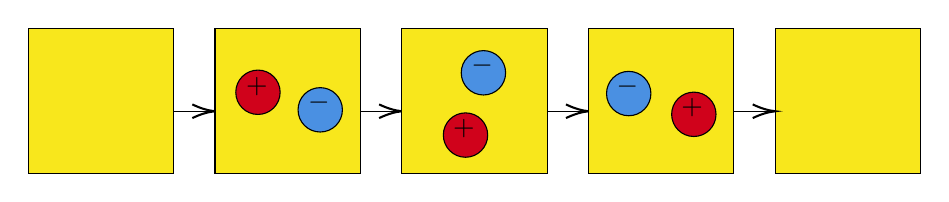
\begin{tikzpicture}[x=0.75pt,y=0.75pt,yscale=-1,xscale=1]
%uncomment if require: \path (0,104); %set diagram left start at 0, and has height of 104

%Shape: Rectangle [id:dp6473613603306763] 
\draw  [fill={rgb, 255:red, 248; green, 231; blue, 28 }  ,fill opacity=1 ] (10,10) -- (80,10) -- (80,80) -- (10,80) -- cycle ;
%Straight Lines [id:da797601032115151] 
\draw    (80,50) -- (98,50) ;
\draw [shift={(100,50)}, rotate = 180] [color={rgb, 255:red, 0; green, 0; blue, 0 }  ][line width=0.75]    (10.93,-3.29) .. controls (6.95,-1.4) and (3.31,-0.3) .. (0,0) .. controls (3.31,0.3) and (6.95,1.4) .. (10.93,3.29)   ;
%Shape: Rectangle [id:dp6852641801099257] 
\draw  [fill={rgb, 255:red, 248; green, 231; blue, 28 }  ,fill opacity=1 ] (100,10) -- (170,10) -- (170,80) -- (100,80) -- cycle ;
%Shape: Ellipse [id:dp6711359850260148] 
\draw  [fill={rgb, 255:red, 208; green, 2; blue, 27 }  ,fill opacity=1 ] (110,40.86) .. controls (110,34.96) and (114.78,30.17) .. (120.68,30.17) .. controls (126.58,30.17) and (131.37,34.96) .. (131.37,40.86) .. controls (131.37,46.76) and (126.58,51.54) .. (120.68,51.54) .. controls (114.78,51.54) and (110,46.76) .. (110,40.86) -- cycle ;

%Shape: Ellipse [id:dp4660922965086378] 
\draw  [fill={rgb, 255:red, 74; green, 144; blue, 226 }  ,fill opacity=1 ] (140,49.32) .. controls (140,43.42) and (144.78,38.63) .. (150.68,38.63) .. controls (156.58,38.63) and (161.37,43.42) .. (161.37,49.32) .. controls (161.37,55.22) and (156.58,60) .. (150.68,60) .. controls (144.78,60) and (140,55.22) .. (140,49.32) -- cycle ;

%Straight Lines [id:da6728827873499814] 
\draw    (170,50) -- (188,50) ;
\draw [shift={(190,50)}, rotate = 180] [color={rgb, 255:red, 0; green, 0; blue, 0 }  ][line width=0.75]    (10.93,-3.29) .. controls (6.95,-1.4) and (3.31,-0.3) .. (0,0) .. controls (3.31,0.3) and (6.95,1.4) .. (10.93,3.29)   ;
%Shape: Rectangle [id:dp456247521401133] 
\draw  [fill={rgb, 255:red, 248; green, 231; blue, 28 }  ,fill opacity=1 ] (190,10) -- (260,10) -- (260,80) -- (190,80) -- cycle ;
%Shape: Ellipse [id:dp6395166789877584] 
\draw  [fill={rgb, 255:red, 208; green, 2; blue, 27 }  ,fill opacity=1 ] (210,61.47) .. controls (210,55.57) and (214.78,50.79) .. (220.68,50.79) .. controls (226.58,50.79) and (231.37,55.57) .. (231.37,61.47) .. controls (231.37,67.37) and (226.58,72.16) .. (220.68,72.16) .. controls (214.78,72.16) and (210,67.37) .. (210,61.47) -- cycle ;

%Shape: Ellipse [id:dp8450181846668086] 
\draw  [fill={rgb, 255:red, 74; green, 144; blue, 226 }  ,fill opacity=1 ] (218.63,31.47) .. controls (218.63,25.57) and (223.42,20.79) .. (229.32,20.79) .. controls (235.22,20.79) and (240,25.57) .. (240,31.47) .. controls (240,37.37) and (235.22,42.16) .. (229.32,42.16) .. controls (223.42,42.16) and (218.63,37.37) .. (218.63,31.47) -- cycle ;

%Straight Lines [id:da5749953405054897] 
\draw    (260,50) -- (278,50) ;
\draw [shift={(280,50)}, rotate = 180] [color={rgb, 255:red, 0; green, 0; blue, 0 }  ][line width=0.75]    (10.93,-3.29) .. controls (6.95,-1.4) and (3.31,-0.3) .. (0,0) .. controls (3.31,0.3) and (6.95,1.4) .. (10.93,3.29)   ;
%Shape: Rectangle [id:dp8134729787266461] 
\draw  [fill={rgb, 255:red, 248; green, 231; blue, 28 }  ,fill opacity=1 ] (280,10) -- (350,10) -- (350,80) -- (280,80) -- cycle ;
%Shape: Ellipse [id:dp5212553581587995] 
\draw  [fill={rgb, 255:red, 208; green, 2; blue, 27 }  ,fill opacity=1 ] (320,51.47) .. controls (320,45.57) and (324.78,40.79) .. (330.68,40.79) .. controls (336.58,40.79) and (341.37,45.57) .. (341.37,51.47) .. controls (341.37,57.37) and (336.58,62.16) .. (330.68,62.16) .. controls (324.78,62.16) and (320,57.37) .. (320,51.47) -- cycle ;

%Shape: Ellipse [id:dp11814790762656346] 
\draw  [fill={rgb, 255:red, 74; green, 144; blue, 226 }  ,fill opacity=1 ] (288.63,41.47) .. controls (288.63,35.57) and (293.42,30.79) .. (299.32,30.79) .. controls (305.22,30.79) and (310,35.57) .. (310,41.47) .. controls (310,47.37) and (305.22,52.16) .. (299.32,52.16) .. controls (293.42,52.16) and (288.63,47.37) .. (288.63,41.47) -- cycle ;

%Shape: Rectangle [id:dp03809290743825433] 
\draw  [fill={rgb, 255:red, 248; green, 231; blue, 28 }  ,fill opacity=1 ] (370,10) -- (440,10) -- (440,80) -- (370,80) -- cycle ;
%Straight Lines [id:da4431173323777904] 
\draw    (350,50) -- (368,50) ;
\draw [shift={(370,50)}, rotate = 180] [color={rgb, 255:red, 0; green, 0; blue, 0 }  ][line width=0.75]    (10.93,-3.29) .. controls (6.95,-1.4) and (3.31,-0.3) .. (0,0) .. controls (3.31,0.3) and (6.95,1.4) .. (10.93,3.29)   ;

% Text Node
\draw (143.58,40.24) node [anchor=north west][inner sep=0.75pt]    {$-$};
% Text Node
\draw (222.21,22.4) node [anchor=north west][inner sep=0.75pt]    {$-$};
% Text Node
\draw (213.45,52.4) node [anchor=north west][inner sep=0.75pt]    {$+$};
% Text Node
\draw (292.21,32.4) node [anchor=north west][inner sep=0.75pt]    {$-$};
% Text Node
\draw (323.45,42.4) node [anchor=north west][inner sep=0.75pt]    {$+$};
% Text Node
\draw (113.7,32.4) node [anchor=north west][inner sep=0.75pt]    {$+$};


\end{tikzpicture}
  \end{center}
  
\end{frame}
\begin{frame}{What about cobordism?}

If we put the movement in 3D space:
\begin{columns}
  
\column{0.5\linewidth}
\centering
\tikzset{every picture/.style={line width=0.75pt}} %set default line width to 0.75pt        

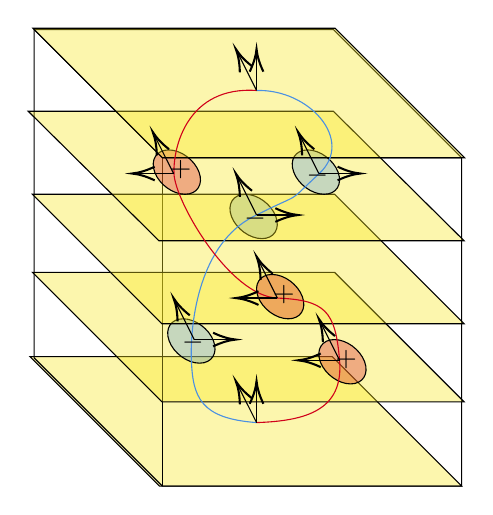
\begin{tikzpicture}[x=0.75pt,y=0.75pt,yscale=-1,xscale=1]
%uncomment if require: \path (0,300); %set diagram left start at 0, and has height of 300

%Shape: Parallelogram [id:dp2829313780044411] 
\draw  [fill={rgb, 255:red, 248; green, 231; blue, 28 }  ,fill opacity=0.36 ] (206.42,188.2) -- (60.82,188.2) -- (123.22,250.6) -- (268.82,250.6) -- cycle ;
%Shape: Cube [id:dp7986901211428024] 
\draw   (268.82,92.4) -- (207.02,30.6) -- (62.82,30.6) -- (62.82,188.8) -- (124.62,250.6) -- (268.82,250.6) -- cycle ; \draw   (62.82,30.6) -- (124.62,92.4) -- (268.82,92.4) ; \draw   (124.62,92.4) -- (124.62,250.6) ;
%Shape: Parallelogram [id:dp5255134756222861] 
\draw  [fill={rgb, 255:red, 248; green, 231; blue, 28 }  ,fill opacity=0.36 ] (207.6,147.6) -- (62,147.6) -- (124.4,210) -- (270,210) -- cycle ;
%Shape: Ellipse [id:dp4175265135497843] 
\draw  [fill={rgb, 255:red, 208; green, 2; blue, 27 }  ,fill opacity=0.3 ] (200.7,190.68) .. controls (198.53,184.78) and (201.55,180) .. (207.46,180) .. controls (213.36,180) and (219.9,184.78) .. (222.07,190.68) .. controls (224.24,196.58) and (221.22,201.37) .. (215.32,201.37) .. controls (209.42,201.37) and (202.88,196.58) .. (200.7,190.68) -- cycle ;

%Shape: Ellipse [id:dp7754560794198566] 
\draw  [fill={rgb, 255:red, 74; green, 144; blue, 226 }  ,fill opacity=0.3 ] (127.91,180.68) .. controls (125.71,174.78) and (128.71,170) .. (134.62,170) .. controls (140.52,170) and (147.08,174.78) .. (149.28,180.68) .. controls (151.48,186.58) and (148.48,191.37) .. (142.57,191.37) .. controls (136.67,191.37) and (130.11,186.58) .. (127.91,180.68) -- cycle ;

%Shape: Parallelogram [id:dp6450713130827144] 
\draw  [fill={rgb, 255:red, 248; green, 231; blue, 28 }  ,fill opacity=0.36 ] (207.6,110) -- (62,110) -- (124.4,172.4) -- (270,172.4) -- cycle ;
%Shape: Ellipse [id:dp6943422388144511] 
\draw  [fill={rgb, 255:red, 74; green, 144; blue, 226 }  ,fill opacity=0.3 ] (157.91,120.68) .. controls (155.71,114.78) and (158.71,110) .. (164.62,110) .. controls (170.52,110) and (177.08,114.78) .. (179.28,120.68) .. controls (181.48,126.58) and (178.48,131.37) .. (172.57,131.37) .. controls (166.67,131.37) and (160.11,126.58) .. (157.91,120.68) -- cycle ;

%Shape: Ellipse [id:dp7158020602917834] 
\draw  [fill={rgb, 255:red, 208; green, 2; blue, 27 }  ,fill opacity=0.3 ] (170.7,159.32) .. controls (168.53,153.42) and (171.55,148.63) .. (177.46,148.63) .. controls (183.36,148.63) and (189.9,153.42) .. (192.07,159.32) .. controls (194.24,165.22) and (191.22,170) .. (185.32,170) .. controls (179.42,170) and (172.88,165.22) .. (170.7,159.32) -- cycle ;

%Shape: Parallelogram [id:dp6566271828309365] 
\draw  [fill={rgb, 255:red, 248; green, 231; blue, 28 }  ,fill opacity=0.36 ] (207,70) -- (60,70) -- (123,132.4) -- (270,132.4) -- cycle ;
%Shape: Ellipse [id:dp3125219871354805] 
\draw  [fill={rgb, 255:red, 208; green, 2; blue, 27 }  ,fill opacity=0.3 ] (120.92,99.32) .. controls (118.75,93.42) and (121.77,88.63) .. (127.67,88.63) .. controls (133.57,88.63) and (140.12,93.42) .. (142.29,99.32) .. controls (144.46,105.22) and (141.44,110) .. (135.54,110) .. controls (129.64,110) and (123.09,105.22) .. (120.92,99.32) -- cycle ;

%Shape: Ellipse [id:dp9355337572596321] 
\draw  [fill={rgb, 255:red, 74; green, 144; blue, 226 }  ,fill opacity=0.3 ] (187.91,99.32) .. controls (185.71,93.42) and (188.71,88.63) .. (194.62,88.63) .. controls (200.52,88.63) and (207.08,93.42) .. (209.28,99.32) .. controls (211.48,105.22) and (208.48,110) .. (202.57,110) .. controls (196.67,110) and (190.11,105.22) .. (187.91,99.32) -- cycle ;

%Shape: Parallelogram [id:dp42810300394364265] 
\draw  [fill={rgb, 255:red, 248; green, 231; blue, 28 }  ,fill opacity=0.36 ] (207.82,30) -- (62.22,30) -- (124.62,92.4) -- (270.22,92.4) -- cycle ;
%Curve Lines [id:da48854427697824443] 
\draw [color={rgb, 255:red, 74; green, 144; blue, 226 }  ,draw opacity=1 ]   (170,220) .. controls (143,218) and (139.19,207.92) .. (138.59,189.32) .. controls (137.99,170.72) and (142.81,133.68) .. (168.59,120.68) .. controls (194.38,107.68) and (183,116) .. (200.22,100) .. controls (217.43,84) and (195.4,59.2) .. (170,60) ;
%Curve Lines [id:da7957006804793516] 
\draw [color={rgb, 255:red, 208; green, 2; blue, 27 }  ,draw opacity=1 ]   (170,220) .. controls (194,219.2) and (212,214) .. (210,190) .. controls (208,166) and (203,161) .. (180,160) .. controls (157,159) and (130.65,113.35) .. (130.22,100) .. controls (129.78,86.65) and (137,57.8) .. (170,60) ;
%Straight Lines [id:da8213826161349653] 
\draw    (200,100) -- (190.89,81.79) ;
\draw [shift={(190,80)}, rotate = 63.43] [color={rgb, 255:red, 0; green, 0; blue, 0 }  ][line width=0.75]    (10.93,-3.29) .. controls (6.95,-1.4) and (3.31,-0.3) .. (0,0) .. controls (3.31,0.3) and (6.95,1.4) .. (10.93,3.29)   ;
%Straight Lines [id:da4206663217899813] 
\draw    (200,100) -- (218,100) ;
\draw [shift={(220,100)}, rotate = 180] [color={rgb, 255:red, 0; green, 0; blue, 0 }  ][line width=0.75]    (10.93,-3.29) .. controls (6.95,-1.4) and (3.31,-0.3) .. (0,0) .. controls (3.31,0.3) and (6.95,1.4) .. (10.93,3.29)   ;

%Straight Lines [id:da6829683618913758] 
\draw    (170,120) -- (160.89,101.79) ;
\draw [shift={(160,100)}, rotate = 63.43] [color={rgb, 255:red, 0; green, 0; blue, 0 }  ][line width=0.75]    (10.93,-3.29) .. controls (6.95,-1.4) and (3.31,-0.3) .. (0,0) .. controls (3.31,0.3) and (6.95,1.4) .. (10.93,3.29)   ;
%Straight Lines [id:da04181480795641934] 
\draw    (170,120) -- (188,120) ;
\draw [shift={(190,120)}, rotate = 180] [color={rgb, 255:red, 0; green, 0; blue, 0 }  ][line width=0.75]    (10.93,-3.29) .. controls (6.95,-1.4) and (3.31,-0.3) .. (0,0) .. controls (3.31,0.3) and (6.95,1.4) .. (10.93,3.29)   ;

%Straight Lines [id:da6390346330114314] 
\draw    (140,180) -- (130.89,161.79) ;
\draw [shift={(130,160)}, rotate = 63.43] [color={rgb, 255:red, 0; green, 0; blue, 0 }  ][line width=0.75]    (10.93,-3.29) .. controls (6.95,-1.4) and (3.31,-0.3) .. (0,0) .. controls (3.31,0.3) and (6.95,1.4) .. (10.93,3.29)   ;
%Straight Lines [id:da9267664003023888] 
\draw    (140,180) -- (158,180) ;
\draw [shift={(160,180)}, rotate = 180] [color={rgb, 255:red, 0; green, 0; blue, 0 }  ][line width=0.75]    (10.93,-3.29) .. controls (6.95,-1.4) and (3.31,-0.3) .. (0,0) .. controls (3.31,0.3) and (6.95,1.4) .. (10.93,3.29)   ;

%Straight Lines [id:da8683444534006999] 
\draw    (130,100) -- (120.89,81.79) ;
\draw [shift={(120,80)}, rotate = 63.43] [color={rgb, 255:red, 0; green, 0; blue, 0 }  ][line width=0.75]    (10.93,-3.29) .. controls (6.95,-1.4) and (3.31,-0.3) .. (0,0) .. controls (3.31,0.3) and (6.95,1.4) .. (10.93,3.29)   ;
%Straight Lines [id:da7147547632524447] 
\draw    (130,100) -- (112,100) ;
\draw [shift={(110,100)}, rotate = 360] [color={rgb, 255:red, 0; green, 0; blue, 0 }  ][line width=0.75]    (10.93,-3.29) .. controls (6.95,-1.4) and (3.31,-0.3) .. (0,0) .. controls (3.31,0.3) and (6.95,1.4) .. (10.93,3.29)   ;

%Straight Lines [id:da7193222744870296] 
\draw    (170,60) -- (160.89,41.79) ;
\draw [shift={(160,40)}, rotate = 63.43] [color={rgb, 255:red, 0; green, 0; blue, 0 }  ][line width=0.75]    (10.93,-3.29) .. controls (6.95,-1.4) and (3.31,-0.3) .. (0,0) .. controls (3.31,0.3) and (6.95,1.4) .. (10.93,3.29)   ;
%Straight Lines [id:da5058086459305744] 
\draw    (170,60) -- (170,42) ;
\draw [shift={(170,40)}, rotate = 90] [color={rgb, 255:red, 0; green, 0; blue, 0 }  ][line width=0.75]    (10.93,-3.29) .. controls (6.95,-1.4) and (3.31,-0.3) .. (0,0) .. controls (3.31,0.3) and (6.95,1.4) .. (10.93,3.29)   ;

%Straight Lines [id:da21485101615353686] 
\draw    (210,190) -- (200.89,171.79) ;
\draw [shift={(200,170)}, rotate = 63.43] [color={rgb, 255:red, 0; green, 0; blue, 0 }  ][line width=0.75]    (10.93,-3.29) .. controls (6.95,-1.4) and (3.31,-0.3) .. (0,0) .. controls (3.31,0.3) and (6.95,1.4) .. (10.93,3.29)   ;
%Straight Lines [id:da819887079574181] 
\draw    (210,190) -- (192,190) ;
\draw [shift={(190,190)}, rotate = 360] [color={rgb, 255:red, 0; green, 0; blue, 0 }  ][line width=0.75]    (10.93,-3.29) .. controls (6.95,-1.4) and (3.31,-0.3) .. (0,0) .. controls (3.31,0.3) and (6.95,1.4) .. (10.93,3.29)   ;

%Straight Lines [id:da907977701793039] 
\draw    (180,160) -- (170.89,141.79) ;
\draw [shift={(170,140)}, rotate = 63.43] [color={rgb, 255:red, 0; green, 0; blue, 0 }  ][line width=0.75]    (10.93,-3.29) .. controls (6.95,-1.4) and (3.31,-0.3) .. (0,0) .. controls (3.31,0.3) and (6.95,1.4) .. (10.93,3.29)   ;
%Straight Lines [id:da5019711894013863] 
\draw    (180,160) -- (162,160) ;
\draw [shift={(160,160)}, rotate = 360] [color={rgb, 255:red, 0; green, 0; blue, 0 }  ][line width=0.75]    (10.93,-3.29) .. controls (6.95,-1.4) and (3.31,-0.3) .. (0,0) .. controls (3.31,0.3) and (6.95,1.4) .. (10.93,3.29)   ;

%Straight Lines [id:da16885377224273834] 
\draw    (170,220) -- (160.89,201.79) ;
\draw [shift={(160,200)}, rotate = 63.43] [color={rgb, 255:red, 0; green, 0; blue, 0 }  ][line width=0.75]    (10.93,-3.29) .. controls (6.95,-1.4) and (3.31,-0.3) .. (0,0) .. controls (3.31,0.3) and (6.95,1.4) .. (10.93,3.29)   ;
%Straight Lines [id:da15238718584339161] 
\draw    (170,220) -- (170,202) ;
\draw [shift={(170,200)}, rotate = 90] [color={rgb, 255:red, 0; green, 0; blue, 0 }  ][line width=0.75]    (10.93,-3.29) .. controls (6.95,-1.4) and (3.31,-0.3) .. (0,0) .. controls (3.31,0.3) and (6.95,1.4) .. (10.93,3.29)   ;


% Text Node
\draw (126.92,92.4) node [anchor=north west][inner sep=0.75pt]    {$+$};
% Text Node
\draw (192.84,95.4) node [anchor=north west][inner sep=0.75pt]    {$-$};
% Text Node
\draw (162.84,115.77) node [anchor=north west][inner sep=0.75pt]    {$-$};
% Text Node
\draw (176.7,152.4) node [anchor=north west][inner sep=0.75pt]    {$+$};
% Text Node
\draw (206.7,183.77) node [anchor=north west][inner sep=0.75pt]    {$+$};
% Text Node
\draw (132.84,175.77) node [anchor=north west][inner sep=0.75pt]    {$-$};


\end{tikzpicture}



\pause
\column{0.5\linewidth}
This provides a framed circle, meaning an embedding $\mathbb{S}^1 \hookrightarrow \mathbb{R}^n$ with a \textbf{ trivialization } $\tau$ of the normal bundle. We denote $\Omega^{fr}_i$ as the group of cobordism classes of $i$-dimensional framed manifolds. \pause And we also have:

\[
  \Omega^{fr}_i \cong \pi^s_i(\mathbb{S}) 
\]

Therefore, this framed circle is non-trivial and is the generator of $\Omega^{fr}_1$.

\end{columns}
\end{frame}
\begin{frame}{Thank you, hope you have got the brain upgrades!}
  
\begin{figure}
  \begin{center}
    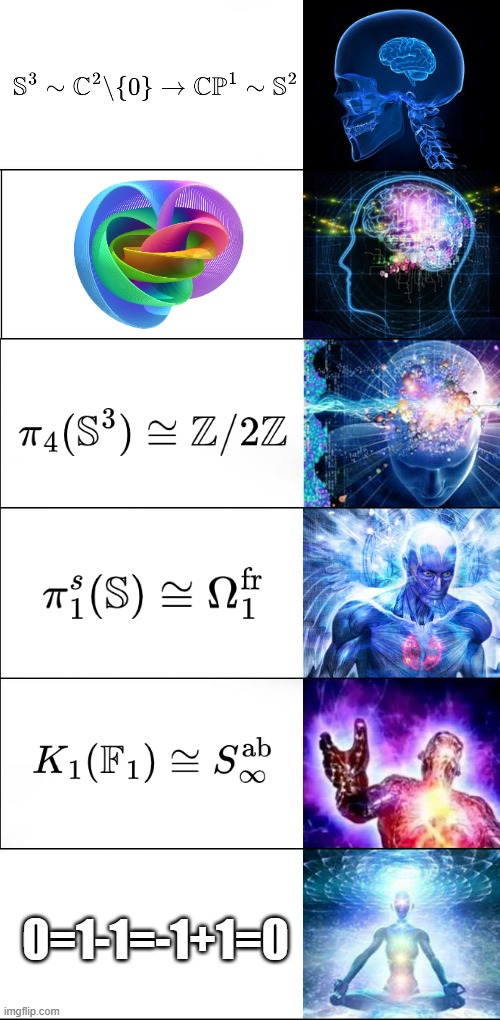
\includegraphics[height=0.8\textheight]{figures/hopf_meme.jpg}
  \end{center}
\end{figure}

\end{frame}
\end{document}
